\documentclass[contribution]{jfsma}

\usepackage[T1]{fontenc}
\usepackage{graphicx}
%\usepackage{color}
%\renewcommand\UrlFont{\color{blue}\rmfamily}
\usepackage{amsthm}
\usepackage{amsmath,amssymb,amsfonts}
\usepackage{tabularx}
\usepackage{caption}
\usepackage{listings}
% \usepackage{titlesec}
% \usepackage[english]{babel}  
% \captionsetup{font=it}
\usepackage{ragged2e}
\usepackage{xurl}
\usepackage{hyperref}
\renewcommand{\figureautorefname}{Figure}
\renewcommand{\tableautorefname}{Table}
% \renewcommand{\equationautorefname}{Équation}
% \renewcommand{\sectionautorefname}{Section}
% \renewcommand{\subsectionautorefname}{Sous-section}
% \renewcommand{\subsubsectionautorefname}{Sous-sous-section}
\usepackage{pifont}
\usepackage{footmisc}
\usepackage{multirow}
\usepackage{enumitem}
\usepackage{algorithm2e}
\usepackage{float}
\usepackage{listings}
\usepackage{xcolor}
% \usepackage[inline, shortlabels]{enumitem}
% \usepackage[hyphens]{url}

\definecolor{codegreen}{rgb}{0,0.6,0}
\definecolor{codegray}{rgb}{0.5,0.5,0.5}
\definecolor{codepurple}{rgb}{0.58,0,0.82}
\definecolor{backcolour}{rgb}{0.95,0.95,0.92}
 
\lstdefinestyle{mystyle}{
    backgroundcolor=\color{backcolour},   
    commentstyle=\color{codegreen},
    keywordstyle=\color{magenta},
    numberstyle=\tiny\color{codegray},
    stringstyle=\color{codepurple},
    basicstyle=\footnotesize,
    breakatwhitespace=false,         
    breaklines=true,                 
    captionpos=b,                    
    keepspaces=true,                 
    numbers=left,                    
    numbersep=5pt,                  
    showspaces=false,                
    showstringspaces=false,
    showtabs=false,                  
    tabsize=2
}
 
\lstset{style=mystyle}

% --- Tickz
\usepackage{physics}
\usepackage{amsmath}
\usepackage{tikz}
\usepackage{mathdots}
\usepackage{yhmath}
\usepackage{cancel}
\usepackage{color}
\usepackage{siunitx}
\usepackage{array}
\usepackage{multirow}
\usepackage{amssymb}
\usepackage{gensymb}
\usepackage{tabularx}
\usepackage{extarrows}
\usepackage{booktabs}
\usetikzlibrary{fadings}
\usetikzlibrary{patterns}
\usetikzlibrary{shadows.blur}
\usetikzlibrary{shapes}

% ---------
% \usepackage{titlesec}
\usepackage{pdfpages}
\usepackage{booktabs}
\usepackage{csquotes}
\usepackage{lipsum}  
\usepackage{arydshln}
\usepackage{smartdiagram}
\usepackage[inkscapeformat=png]{svg}
\usepackage{textcomp}
\usepackage{tabularray}\UseTblrLibrary{varwidth}
\usepackage{xcolor}
\def\BibTeX{{\rm B\kern-.05em{\sc i\kern-.025em b}\kern-.08em
    T\kern-.1667em\lower.7ex\hbox{E}\kern-.125emX}}
\usepackage{cite}
\usepackage{amsmath}
\newcommand{\probP}{\text{I\kern-0.15em P}}
\usepackage{etoolbox}
\patchcmd{\thebibliography}{\section*{\refname}}{}{}{}

\setlength\tabcolsep{0.5pt}

\newcommand{\before}[1]{\textcolor{red}{#1}}
\newcommand{\after}[1]{\textcolor{green}{#1}}

\newcommand{\old}[1]{\textcolor{orange}{#1}}
\newcommand{\rem}[1]{\textcolor{red}{#1}}
\newcommand{\todo}[1]{\textcolor{orange}{\newline \textit{\textbf{TODO:} #1}} \newline \newline }



\newcounter{relation}
\setcounter{relation}{0}
\renewcommand{\therelation}{\arabic{relation}}
\newcommand{\relationautorefname}{Relation}

\newenvironment{relation}[1][]{%
    \refstepcounter{relation}%
    \noindent \raggedright \textit{\textbf{Relation. \therelation}} \hfill$}
{%
$ \hfill \phantom{x}

}

\newcounter{proof}
\setcounter{proof}{0}
\renewcommand{\theproof}{\arabic{proof}}
\newcommand{\proofautorefname}{Proof}

\renewenvironment{proof}[1][]{
    \refstepcounter{proof}
    \noindent \raggedright \textit{\textbf{Proof. \theproof}}

    \setlength{\leftskip}{1em}

}
{

\
\setlength{\leftskip}{0pt}
}

\titre{Une Approche basée sur l'Apprentissage par Renforcement pour l'Ingénierie Organisationelle d'un SMA}


\auteur{Julien Soulé\up{a,b}}{julien.soule@lcis.grenoble-inp.fr}
\auteur{Jean-Paul Jamont\up{a}}{jean-paul.jamont@lcis.grenoble-inp.fr}
\auteur{Michel Occello\up{a}}{michel.occello@lcis.grenoble-inp.fr}
%%%Si besoin d'ajouter des auteurs à la ligne :
\auteurSuite{Louis-Marie Traonouez\up{b}}{louis-marie.traonouez@thalesgroup.com}
\auteurSuite{Paul Théron\up{c}}{paul.theron@orange.fr}

\institution{\up{a}%
  Univ. Grenoble Alpes, Grenoble INP, LCIS, 26000, Valence, France}
\institution{\up{b}%
  Thales Land and Air Systems, BL IAS, Rennes, France}
\institution{\up{c}%
  AICA IWG, La Guillermie, France}

% TODO: est-ce qu'on peut utiliser "dissemination" alors que le papier AIAI n'est pas publié à proprement parler?

\begin{document}

\maketitle

\begin{resume}

  Les SMAs de Cyberdéfense doivent assurer la protection de systèmes en réseau hétérogènes et distribués allant de la détection d’anomalies à l’exécution de contre-mesures. 
  %
  L’organisation est au cœur de ces SMAs et impacte la façon dont les agents interagissent entre eux et avec leur environnement pour favoriser l’atteinte d’un objectif de Cyberdéfense tout en satisfaisant les contraintes de l’environnement.
  %
  Néanmoins, la complexité et le manque de lisibilité de certains environnements rendent difficile et non sûre une recherche empirique d’une organisation adaptée.
  %
  La recherche d’une organisation adéquate est un problème  rencontré pour la conception de la plupart des SMAs et dépasse la problématique de ces applications spécifiques.
  %
  Cet article propose une approche générique et un outil permettant de faciliter la conception de l’organisation en combinant un processus d’apprentissage par renforcement et un modèle organisationnel. L’outil suggère des spécifications organisationnelles pour aider le concepteur.
  
\end{resume}

\motscles{Organisations, Ingénierie multi-agents, Simulation multi-agents, Apprentissage multi-agent}

\bigskip

\begin{abstract}

  The Cyberdefense MASs must ensure the protection of heterogeneous and distributed networked systems ranging from anomaly detection to countermeasure execution.
  %
  Organization lies at the core of these MASs and impacts how agents interact and with their environment to foster the achievement of a Cyberdefense objective while meeting the constraints of the environment.
  %
  However, the complexity and lack of readability of some environments make difficult and unsafe an empirical search for a suitable organization.
  %
  The search for an adequate organization is a problem encountered in the design of most MASs and goes beyond the issues of these specific applications.
  %
  This article proposes a generic approach and a tool to facilitate the organization's design by combining a reinforcement learning process and an organizational model. The tool suggests organizational specifications to help the designer.
\end{abstract}

\keywords{Organizations, Multi-agent engineering, Multi-agent simulation, Multi-agent learning}

\section{Introduction}

% Contexte:

%% Introduire le concept de SMA de Cyberdefense en le supportant par l'AICA
Les SMAs de Cyberdéfense~\cite{Kott2023, Singh2015} doivent assurer la protection d'environnements cyber-pyhysiques complexes.  La détection et l'identification des attaques sont essentielles pour raisonner sur les menaces en cours, tandis que l'élaboration et l'exécution des contre-mesures permettent de répondre efficacement à ces menaces et de minimiser les dommages potentiels. Dans ce contexte, le groupe \emph{AICA International Work Group} a proposé l'\emph{Autonomous Intelligent Cyberdefense Agent} (AICA)
\footnote{La recherche sur les AICA a été initiée le cadre du groupe \emph{NATO IST-152} puis de l'\emph{AICA International Work Group} : \url{https://www.aica-iwg.org/}. }
qui peut être vu comme un SMA de Cyberdéfense. L'ingénierie du SMA de Cyberdéfense a été identifiée par ce groupe de travail comme un défi important, en particulier pour ce qui concerne les aspects organisationnels. % est mise en avant en raison notamment du manque de compréhension visuelle et intuitive des environnements en réseau et de leurs spécificités propres.
Un tel système doit être performant contre les attaques malgré les contraintes environnementales. Il peut notamment renforcer sa résilience en favorisant par exemple la redondance, la diversité, l'autonomie et l'adaptabilité de ses composants et de ses interactions.

% L'organisation d'un tel système doit en effet renforcer sa résilience en favorisant par exemple la redondance, la diversité, l'autonomie et l'adaptabilité de ses composants et de ses interactions.
% -> JS : Trop tôt pour parler d'organisation. On peut vouloir un SMA capable de s'adapter sans le voir au travers du prisme de l'organisation nécessairement, non ?

%% Elargir le sujet des SMAC/AICA au contexte des SMA en général
Au-delà du contexte de la cyberdéfense, la conception d'un SMA repose sur les démarches proposées dans des méthodes de conception telles que GAIA~\cite{Wooldridge2000,Cernuzzi2014}, ADELFE~\cite{Mefteh2015}, MaSE~\cite{Deloach2001}, DIAMOND~\cite{Jamont2015} ou KB-ORG~\cite{Sims2008}.
Ces méthodes reposent généralement sur un processus itératif procédant par essais et erreurs guidés par l'expérience du concepteur pour élaborer la logique interne des agents. Cependant, la complexité et le manque de connaissance des systèmes cibles peuvent rendre coûteuse l'application de ces méthodes et ne garantissent pas de converger vers un SMA répondant aux exigences de performance~\cite{Mefteh2013}.


% Problème en 2 temps : 
% - l'organisation comme moyen de poser la problématique de conception comme un problème d'optimisation sous contraintes
% - le constat qu'il n'existe pas de méthode pour générer une organisation de façon automatisée sans connaissance préalables

Le concept d'organisation se réfère à la fois aux agents à travers leurs logiques internes et aux supports explicitant comment les agents coordonnent leurs activités pour atteindre de manière collaborative un objectif commun~\cite{Picard2009}. L'organisation occupe une place fondamentale dans la conception du SMA.
%
% JS : "L'organisation, qui désigne la structure et les règles qui..."
% -> En fait je pense que cette phrase confond l'organisation et le support de l'organisation: On ne peut pas résumer l'organisation à des structures, fonctions... cela n'en est simplement que la représentation...
%
% De mon point de vue:
% - les seules choses qui existent véritablement sont les agents et leur comportements issus de leurs logiques internes (règles).
% - l'ensemble des agents forment l'entité de l'organisation (cf. Gauthier Picard) dans le sens où l'on est sûr que l'organisation est "contenue" dans les agents même si on ne cherche pas nécéssairement à rendre l'organisation explicite
% - cette entité de l'organisation (ou organisation) peut être explicitée au travers d'un support (modèle organisationel) qui met éventuellement en jeu des structures (roles...), fonctions...
%
% -> Même si tu prends des SMAs centrés organisation et conscients de l'organisation (cf. Gauthier Picard), cette vision reste valable:
% -> Si on prend des agents qui partageraient une représentation commune de l'organisation et qui pourraient la manipuler, on ne peut pas dire que l'ensemble des agents sont strictement égaux à leur représentation
%
%
Dans ce travail, nous abordons la conception d'un SMA comme un problème d’optimisation consistant à trouver l’organisation qui satisfait les contraintes de déploiement de l’environnement et qui favorise la meilleure performance dans l’atteinte d’un objectif.
En utilisant des connaissances prédéfinies, certaines méthodes pourraient automatiser certaines parties de la recherche d'une organisation de SMA appropriée, comme KB-ORG~\cite{Sims2008}.

Cependant, il n'y a aucun moyen agnostique de l'environnement cible permettant d'automatiser totalement la recherche des logiques internes des agents (que nous appelons également \textbf{politiques}) qui satisfait les exigences données tout en explicitant les mécanismes organisationnels. %émergents. -> JS : j'enlève "émergent" car les mecanismes organisationels ne sont pas tous émérgents. Certains sont intentionellement voulus.

% Contribution : On introduit AOMEA en résumant cela comme Résolution du pb en jouant sur les politiques des agents + interpretation en spec. org. pour la conception
Nous introduisons \emph{AOMEA} (Assisted Multi-Agent System Organization Engineering Approach), une approche de conception SMA dont l'idée sous-jacente est de lier un processus \emph{Multi-Agent Reinforcement Learning} donné à un modèle organisationnel qui relie les politiques des agents entrainés à des spécifications organisationnelles explicites. Ainsi, pour des agents entrainés répondant aux exigences données, les spécifications organisationnelles associées peuvent suggérer au concepteur des mécanismes organisationnels à mettre en place pour développer un SMA adéquat.% vis à vis de son objectif et les contraintes données.

% Résultats

% Nous avons appliqué AOMEA dans trois jeux Atari spatiaux avec différents degrés de coopération requis entre les agents afin qu'ils atteignent un objectif le plus efficacement possible ; et en outre en respectant les spécifications organisationnelles comme contraintes de conception. Les spécifications organisationnelles obtenues sont en effet exploitables, cohérentes avec les attentes et respectent les contraintes de conception.
%Nous avons également appliqué notre approche, dans un environnement d'essaim de drones de Cyberdéfense dont les spécifications organisationnelles résultantes ont conduit à développer un SMA avec des scores comparables aux principaux.

La section II commence par présenter les concepts fondamentaux d'AOMEA que nous utilisons pour lier le modèle organisationnel et MARL.
% et la motivation pour intégrer un modèle organisationnel SMA dans un processus MARL afin d'améliorer le processus de conception SMA.
Dans la section III, nous présentons AOMEA depuis l’approche jusqu’à l’outil mis en œuvre. Nous avons évalué AOMEA dans quatre environnements simulés et nous discutons des résultats obtenus dans la section IV. Enfin, la section V conclut sur la viabilité d'AOMEA et met en évidence les limitations et les travaux futurs.

% ================================================== =================================================== =

\section{Cadre théorique}

% // Mettre en avant les briques du raisonnement en raison du titre pour préparer l'introduction de la contribution avec AOMEA sans les justifier (sans faire de comparaison avec l'existant, pas d'édt, dire juste les points forts)

% Organisation
% -> moise (justificateur parmi les existants)

% Méthodologies SMA (ALAADIN, GAIAI mais pas de moyens pour trouver une organisation automatiquemenet)

% MARL (basiques) // DECPOMDP (basiques)

Nous présentons les bases du modèle organisationnel $\mathcal{M}OISE^+$ et les bases MARL sur lesquelles est construite notre contribution.

\subsection{Le modèle organisationnel  MOISE+}

% définition, modèle AEIO, focus Moise, Dec-POMDP

% Un agent est une entité immergée dans un environnement qui perçoit l'observation et prend la décision d'agir de manière autonome dans l'environnement pour atteindre les objectifs qui lui sont assignés.
% Les types d'agents incluent des agents réactifs pilotés par les événements pour gérer les incertitudes dans un environnement ou des agents cognitifs proactifs qui exploitent les interactions avec d'autres agents. Un SMA est un ensemble d'agents dans un environnement partagé où chaque agent n'a qu'une perception locale. Ces agents doivent être dotés de capacités d'auto/réorganisation qui leur permettent de modifier de manière adaptative leur structure organisationnelle en fonction de leur environnement.

Un SMA est fortement lié à l'entité de l'organisation (ou simplement \textbf{organisation}) que nous considérons toujours exister à travers les interactions des agents en cours d'exécution même si elle peut être implicite.
%
% Ces méthodes sont essentielles pour garantir que SMA puisse coordonner, communiquer et exécuter efficacement des tâches dans un environnement distribué et souvent dynamique.
% Les méthodes les plus remarquables incluent
% \emph{Tropos} qui est une méthodologie de développement logiciel orientée agent qui met l'accent sur l'analyse précoce des exigences et l'affinement continu de ces exigences tout au long des phases de conception et de mise en œuvre~\cite{Bresciani2004} ;
% \emph{Gaia}, une méthodologie pour l'analyse et la conception de SMA, axée sur la structure organisationnelle du système~\cite{Zambonelli2003} ; \emph{DIAMOND} qui s'appuie sur une approche itérative en quatre phases pour améliorer le développement de systèmes physiques multi-agents ; et {ADELFE} qui utilisent les compétences et les attitudes lors de la conception pour créer des systèmes auto-organisés et répondre aux exigences finales.
% Dans le cadre des travaux méthodologiques, il convient également de noter le modèle AEIO (Voyelles) qui met l'accent sur la structuration des entités au sein des systèmes multi-agents en incorporant les agents, l'environnement, les interactions et l'organisation comme composants clés.
%
Un \textbf{modèle organisationnel} spécifie (au moins partiellement) l'organisation : si l'organisation est connue explicitement, le modèle organisationnel sert de support à son implémentation ; si l'organisation est émergente, le modèle organisationnel sert de support à sa description. Nous faisons référence aux \textbf{spécifications organisationnelles} comme les composants utilisés dans un modèle organisationnel pour caractériser l'organisation.
En particulier, les notions de rôles, de groupes/équipes, et de normes sont fréquemment utilisées dans les modèles organisationnels.
% tels que AGRE, $\mathcal{M}OISE^+$, OMNI, OperA, and TÆMS~\cite{Lacomme2011}.

% \begin{table}[t!]

    \centering

    \begin{tblr}{colspec={llll},width=\linewidth,row{1}={rowsep=1mm,m},row{2-Z}={rowsep=-1mm,m},measure=vbox,stretch=-10}

        \textbf{ \small Org. Model} & \textbf{ \small Advantages} & \textbf{ \small Limitations} \\

        \hline

        { \small AGRE }
        & { \small Simplici }
        & { \small 4.7 } \\

        \hline[dashed]

        { \small ISLANDER }
        & { \small PPY }
        & { \small 6.3 } \\

        \hline[dashed]

        { \small MOISE+ }
        & { \small KAZ }
        & { \small 4.0 } \\

        \hline[dashed]

        { \small OperA }
        & { \small CYB }
        & { \small 12.0 } \\

        \hline[dashed]

        { \small STEAM }
        & { \small CYB }
        & { \small 12.0 } \\

        \hline[dashed]

        { \small TÆMS }
        & { \small CYB }
        & { \small 12.0 } \\

    \end{tblr}

    \caption{Aperçu des modèles organisationnels}

    \label{tab:organizational_models}

\end{table}


% Les modèles ISLANDER, OMNI ou OperA proposent une approche normative du SMA où les agents sont associés à des rôles de façon dynamique ce qui n'est pas couvert par $\mathcal{M}OISE^+$. Néanmoins, 

$\mathcal{M}OISE^+$~\cite{Hubner2007} permet de lier les politiques des agents à des spécifications organisationnelles. % JS : 
Le cadre complet et formel permet une description détaillée sur les aspects structurels, fonctionnels et normatifs là où \emph{AGRE}~\cite{Ferber2004}, ISLANDER~\cite{Esteva2002}, OMNI~\cite{Dignum2005} ou STEAM~\cite{Tambe1999} peuvent présenter des capacités limitées de description ou sont moins avancées.
% ODML est conçu pour la dynamique organisationnelle des SMA et peut manquer de généricité pour comparer plusieurs SMAs entre eux.
Les modèles STEAM et TÆMS~\cite{Vincent2000} se basent respectivement sur les notions d'équipe et de tâche pour décrire la réponse fonctionnelle du SMA tandis que les aspects normatifs et structurels sont peu couverts.
$\mathcal{M}OISE^+$ considère trois types de spécifications :

Les \textbf{spécifications structurelles} décrivent les moyens que les agents peuvent exploiter pour atteindre un objectif. Elles comprennent l'ensemble des \emph{rôles}, des sous-groupes, des \emph{liens} intra-groupe et inter-groupe, des \emph{compatibilités} intra-groupe et inter-groupe, ainsi que le rôle et le sous-groupe \emph {cardinalités}.
Un \emph{link} indique si deux rôles sont liés en raison de liens de connaissance, de communication ou d'autorité. Une \emph{compatibilité} indique si deux rôles peuvent être adoptés par le même agent. Les \emph{cardinalités} de rôle et de sous-groupe font respectivement référence au nombre minimal et maximal de rôles et de sous-groupes.

Les \textbf{spécifications fonctionnelles} décrivent la manière d'atteindre un objectif. Elles comprennent des \emph{schèmes sociaux} et des \emph{ordres de préférence}. Un \emph{schéma social} est décrit par des objectifs globaux, des étiquettes de mission avec des plans et le cardinal des agents engagés dans une mission. Un \emph{ordre de préférence} signifie qu'un agent a une préférence sociale pour s'engager dans une mission spécifique parmi plusieurs possibles.

Les \textbf{spécifications déontiques} permettent de relier les spécifications fonctionnelles et structurelles à travers un ensemble de \emph{permissions} et d'\emph{obligations}. Une \emph{permission} signifie qu'un agent jouant le rôle $\rho_a$ est autorisé à s'engager dans la mission $m$ pour une contrainte de temps donné $tc$. De même, une \emph{obligation} signifie qu'un agent jouant le rôle $\rho_a$ doit s'engager dans la mission $m$ pour une contrainte de temps donné $tc$. Une contrainte de temps $tc $ spécifie un ensemble de périodes déterminant si une autorisation ou une obligation est valide.

% Pourtant, ces travaux méthodologiques s'appuient largement sur l'expérience des concepteurs humains alors qu'aucun d'entre eux ne permet d'automatiser l'assistance au processus de conception SMA en garantissant une efficacité suffisante tout en prenant en compte les aspects organisationnels dans un contexte multi-agents.

\subsection{L'apprentissage par renforcement multi-agent}

L'apprentissage par renforcement est un paradigme d'apprentissage automatique dans lequel les agents apprennent à prendre des décisions en interagissant avec un environnement. L’objectif est que l’agent maximise la récompense cumulée au fil du temps grâce à un processus d’essais et d’erreurs.
MARL étend ce concept à plusieurs agents qui apprennent simultanément à adapter leurs stratégies tout en considérant les actions et les influences des autres agents. Cela pousse les agents à s’appuyer sur des mécanismes de coopération, de compétition et de coordination.
% JS: c'est pas un trop lourd ? on peut virer manuelle je pense et on garde classique ?
% JS : "classique" ça me parait flou 
MARL permet de converger automatiquement vers les politiques des agents qui permettent d'atteindre l'objectif donné. Pourtant, contrairement à une conception classique, la logique des agents entrainés n'est pas explicitement spécifiée d'un point de vue collectif. Peu de travaux tentent d’aborder cette question et peu sont orientés à des fins méthodologiques.
Kazhdan et. al.~\cite{Kazhdan2020} a proposé des moyens pour extraire des modèles symboliques des systèmes MARL qui améliorent l'interprétabilité des systèmes MARL.
Wang et. al.~\cite{Wang2020} a introduit une approche MARL orientée rôles dans laquelle les rôles sont émergents et les agents ayant des rôles similaires ont tendance à partager leur apprentissage et à se spécialiser dans certaines sous-tâches.
Tosic et. al~\cite{Tosic2010} ont proposé un cadre pour aborder la coordination dans les SMA collaboratifs en s'appuyant sur les capacités de communication des systèmes multi-agents.
Zheng et. al.~\cite{Zheng2018} a présenté une plateforme pour MARL qui vise à faciliter la recherche sur l'intelligence collective artificielle en fournissant un ensemble complet de mesures d'évaluation pour comparer les performances d'algorithmes MARL.

Des modèles Markoviens sont nécessaires pour modéliser l'environnement et appliquer les techniques MARL. En tant qu'outil couramment utilisé, le Dec-POMDP~\cite{Oliehoek2016} considère plusieurs agents de façon analogue à un ensemble. Il s'appuie sur des processus stochastiques pour modéliser l'incertitude de l'environnement pour les changements induits par les actions, les observations reçues, mais aussi les communications. Sa fonction de récompense est commune aux agents ce qui favorise la formation d'actions orientées pour la collaboration~\cite{Beynier2013}. Formellement, un Dec-POMDP est un 7-tuple $(S,\{A_i\},T,R,\{\Omega_i\},O,\gamma)$ , où : $S = \{s_1, .. s_{|S|}\}$ est l''ensemble des états possibles ; $A_{i} = \{a_{1}^{i},..,a_{|A_{i}|}^{i}\}$ l'ensemble des actions possibles pour l'agent $i$ ; $T$ pour que $T(s,a,s') = \probP{(s'|s,a)}$ l'ensemble des probabilités de transition conditionnelles entre les états ; $R : S \times A \times S \rightarrow \mathbb{R}$ la fonction de récompense ; $\Omega_{i} = \{o_{1}^{i},..,o_{|\Omega_{i}|}^{i}\}$  l'ensemble d'observations pour l'agent $ag_i$ ; $O$ pour que $O(s',a,o) = \probP{(o|s',a)}$  l'ensemble des probabilités d'observation conditionnelles ; $\gamma \in [0,1]$, l'horizon.

Nous appelons \textbf{résoudre} le Dec-POMDP pour l'équipe $t$ la recherche d'une politique conjointe $\pi_{joint,i} \in \Pi_{joint}$ qui maximise la récompense cumulée attendue sur un horizon fini.
Nous faisons référence à la \textbf{résolution sous-optimale} du Dec-POMDP à une espérance de $s$ comme étant la recherche des politiques conjointes $\pi_{joint,i} \in \Pi_{joint}$ qui obtiennent la récompense cumulative attendue sur un épisode à une espérance minimale ou égale à $s \in \mathbb{R}$.


% ================================================== =================================================== =

\section{Approche AOMEA}

% Mettre d'abord en avant le shcéma général de l'approche
% Donner la philosophie de l'approche

% 	Aperçu global (Fig. 1)
% 	noyau théorique
% 	Ingénierie
% Implémentation (vers une implémentation de type PoC)

\subsection{Vue d'ensemble}

\begin{figure}[h!]
  \centering
  


\tikzset{every picture/.style={line width=0.75pt}} %set default line width to 0.75pt        

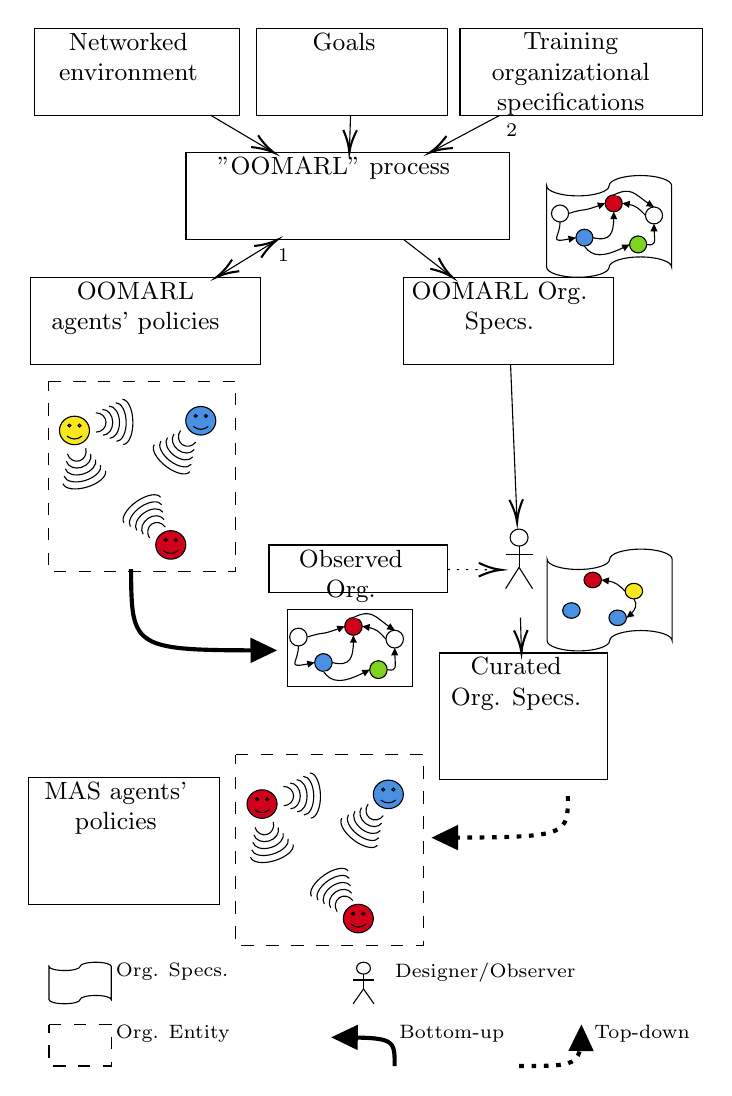
\begin{tikzpicture}[x=0.75pt,y=0.75pt,yscale=-1,xscale=1]
%uncomment if require: \path (0,567); %set diagram left start at 0, and has height of 567

%Flowchart: Punched Tape [id:dp6253416173354658] 
\draw  [fill={rgb, 255:red, 255; green, 255; blue, 255 }  ,fill opacity=1 ] (250,275.87) .. controls (250,278.58) and (256.74,280.77) .. (265.06,280.77) .. controls (273.38,280.77) and (280.12,278.58) .. (280.12,275.87) .. controls (280.12,273.16) and (286.87,270.97) .. (295.18,270.97) .. controls (303.5,270.97) and (310.25,273.16) .. (310.25,275.87) -- (310.25,315.1) .. controls (310.25,312.39) and (303.5,310.19) .. (295.18,310.19) .. controls (286.87,310.19) and (280.12,312.39) .. (280.12,315.1) .. controls (280.12,317.8) and (273.38,320) .. (265.06,320) .. controls (256.74,320) and (250,317.8) .. (250,315.1) -- cycle ;
%Shape: Ellipse [id:dp3141849675822821] 
\draw  [fill={rgb, 255:red, 208; green, 2; blue, 27 }  ,fill opacity=1 ] (267.77,285.83) .. controls (267.77,283.76) and (269.66,282.08) .. (271.98,282.08) .. controls (274.3,282.08) and (276.19,283.76) .. (276.19,285.83) .. controls (276.19,287.9) and (274.3,289.58) .. (271.98,289.58) .. controls (269.66,289.58) and (267.77,287.9) .. (267.77,285.83) -- cycle ;
%Shape: Ellipse [id:dp24618456488955864] 
\draw  [fill={rgb, 255:red, 248; green, 231; blue, 28 }  ,fill opacity=1 ] (287.6,291.19) .. controls (287.6,289.12) and (289.49,287.44) .. (291.81,287.44) .. controls (294.13,287.44) and (296.02,289.12) .. (296.02,291.19) .. controls (296.02,293.27) and (294.13,294.95) .. (291.81,294.95) .. controls (289.49,294.95) and (287.6,293.27) .. (287.6,291.19) -- cycle ;
%Shape: Ellipse [id:dp8783844186516785] 
\draw  [fill={rgb, 255:red, 74; green, 144; blue, 226 }  ,fill opacity=1 ] (279.79,304.06) .. controls (279.79,301.99) and (281.67,300.31) .. (284,300.31) .. controls (286.32,300.31) and (288.2,301.99) .. (288.2,304.06) .. controls (288.2,306.13) and (286.32,307.81) .. (284,307.81) .. controls (281.67,307.81) and (279.79,306.13) .. (279.79,304.06) -- cycle ;
%Curve Lines [id:da8862512396754962] 
\draw [fill={rgb, 255:red, 255; green, 255; blue, 255 }  ,fill opacity=1 ]   (287.6,291.19) .. controls (284.11,287.9) and (283.1,286.97) .. (279.08,286.26) ;
\draw [shift={(276.19,285.83)}, rotate = 7.39] [fill={rgb, 255:red, 0; green, 0; blue, 0 }  ][line width=0.08]  [draw opacity=0] (3.57,-1.72) -- (0,0) -- (3.57,1.72) -- cycle    ;
%Shape: Ellipse [id:dp10865415349748586] 
\draw  [fill={rgb, 255:red, 74; green, 144; blue, 226 }  ,fill opacity=1 ] (257.5,300.55) .. controls (257.5,298.48) and (259.38,296.8) .. (261.71,296.8) .. controls (264.03,296.8) and (265.91,298.48) .. (265.91,300.55) .. controls (265.91,302.62) and (264.03,304.3) .. (261.71,304.3) .. controls (259.38,304.3) and (257.5,302.62) .. (257.5,300.55) -- cycle ;
%Curve Lines [id:da9209146587835657] 
\draw [fill={rgb, 255:red, 255; green, 255; blue, 255 }  ,fill opacity=1 ]   (291.81,294.95) .. controls (293.69,297.65) and (292.57,300.02) .. (290.45,302.13) ;
\draw [shift={(288.2,304.06)}, rotate = 322.38] [fill={rgb, 255:red, 0; green, 0; blue, 0 }  ][line width=0.08]  [draw opacity=0] (3.57,-1.72) -- (0,0) -- (3.57,1.72) -- cycle    ;

%Shape: Rectangle [id:dp5799704037482001] 
\draw  [dash pattern={on 4.5pt off 4.5pt}] (9.63,190) -- (100,190) -- (100,281.94) -- (9.63,281.94) -- cycle ;
%Shape: Smiley Face [id:dp642715493380654] 
\draw  [fill={rgb, 255:red, 248; green, 231; blue, 28 }  ,fill opacity=1 ] (15.05,213.78) .. controls (15.05,209.99) and (18.29,206.92) .. (22.28,206.92) .. controls (26.28,206.92) and (29.51,209.99) .. (29.51,213.78) .. controls (29.51,217.57) and (26.28,220.65) .. (22.28,220.65) .. controls (18.29,220.65) and (15.05,217.57) .. (15.05,213.78) -- cycle ; \draw  [fill={rgb, 255:red, 248; green, 231; blue, 28 }  ,fill opacity=1 ] (19.1,211.45) .. controls (19.1,211.07) and (19.43,210.76) .. (19.82,210.76) .. controls (20.22,210.76) and (20.55,211.07) .. (20.55,211.45) .. controls (20.55,211.83) and (20.22,212.13) .. (19.82,212.13) .. controls (19.43,212.13) and (19.1,211.83) .. (19.1,211.45) -- cycle ; \draw  [fill={rgb, 255:red, 248; green, 231; blue, 28 }  ,fill opacity=1 ] (24.02,211.45) .. controls (24.02,211.07) and (24.34,210.76) .. (24.74,210.76) .. controls (25.14,210.76) and (25.46,211.07) .. (25.46,211.45) .. controls (25.46,211.83) and (25.14,212.13) .. (24.74,212.13) .. controls (24.34,212.13) and (24.02,211.83) .. (24.02,211.45) -- cycle ; \draw   (18.67,216.53) .. controls (21.08,218.36) and (23.49,218.36) .. (25.9,216.53) ;
%Shape: Arc [id:dp7103754459108031] 
\draw  [draw opacity=0] (37.24,233.21) .. controls (37.24,233.21) and (37.24,233.21) .. (37.24,233.21) .. controls (38,235.82) and (34.04,239.33) .. (28.39,241.04) .. controls (22.74,242.76) and (17.53,242.04) .. (16.77,239.43) -- (27,236.32) -- cycle ; \draw   (37.24,233.21) .. controls (37.24,233.21) and (37.24,233.21) .. (37.24,233.21) .. controls (38,235.82) and (34.04,239.33) .. (28.39,241.04) .. controls (22.74,242.76) and (17.53,242.04) .. (16.77,239.43) ;  
%Shape: Arc [id:dp9993647702991559] 
\draw  [draw opacity=0] (34.85,230.5) .. controls (35.62,233.11) and (32.31,236.42) .. (27.46,237.89) .. controls (22.62,239.37) and (18.07,238.44) .. (17.3,235.83) -- (26.08,233.17) -- cycle ; \draw   (34.85,230.5) .. controls (35.62,233.11) and (32.31,236.42) .. (27.46,237.89) .. controls (22.62,239.37) and (18.07,238.44) .. (17.3,235.83) ;  
%Shape: Arc [id:dp33021260729129986] 
\draw  [draw opacity=0] (32.46,227.79) .. controls (32.46,227.79) and (32.46,227.79) .. (32.46,227.79) .. controls (32.46,227.79) and (32.46,227.79) .. (32.46,227.79) .. controls (33.23,230.4) and (30.58,233.51) .. (26.54,234.74) .. controls (22.5,235.97) and (18.61,234.85) .. (17.84,232.24) -- (25.15,230.02) -- cycle ; \draw   (32.46,227.79) .. controls (32.46,227.79) and (32.46,227.79) .. (32.46,227.79) .. controls (32.46,227.79) and (32.46,227.79) .. (32.46,227.79) .. controls (33.23,230.4) and (30.58,233.51) .. (26.54,234.74) .. controls (22.5,235.97) and (18.61,234.85) .. (17.84,232.24) ;  
%Shape: Arc [id:dp7515950702187679] 
\draw  [draw opacity=0] (30.07,225.09) .. controls (30.07,225.09) and (30.07,225.09) .. (30.07,225.09) .. controls (30.07,225.09) and (30.07,225.09) .. (30.07,225.09) .. controls (30.84,227.7) and (28.84,230.61) .. (25.61,231.59) .. controls (22.38,232.57) and (19.14,231.25) .. (18.38,228.64) -- (24.22,226.86) -- cycle ; \draw   (30.07,225.09) .. controls (30.07,225.09) and (30.07,225.09) .. (30.07,225.09) .. controls (30.07,225.09) and (30.07,225.09) .. (30.07,225.09) .. controls (30.84,227.7) and (28.84,230.61) .. (25.61,231.59) .. controls (22.38,232.57) and (19.14,231.25) .. (18.38,228.64) ;  
%Shape: Arc [id:dp17995425823285305] 
\draw  [draw opacity=0] (27.69,222.38) .. controls (27.69,222.38) and (27.69,222.38) .. (27.69,222.38) .. controls (27.69,222.38) and (27.69,222.38) .. (27.69,222.38) .. controls (28.45,224.99) and (27.11,227.7) .. (24.69,228.44) .. controls (22.27,229.18) and (19.68,227.66) .. (18.91,225.05) -- (23.3,223.71) -- cycle ; \draw   (27.69,222.38) .. controls (27.69,222.38) and (27.69,222.38) .. (27.69,222.38) .. controls (27.69,222.38) and (27.69,222.38) .. (27.69,222.38) .. controls (28.45,224.99) and (27.11,227.7) .. (24.69,228.44) .. controls (22.27,229.18) and (19.68,227.66) .. (18.91,225.05) ;  

%Shape: Arc [id:dp8934563741256025] 
\draw  [draw opacity=0] (45.36,198.82) .. controls (48.04,198.76) and (50.3,203.58) .. (50.42,209.59) .. controls (50.54,215.59) and (48.46,220.49) .. (45.78,220.55) -- (45.57,209.68) -- cycle ; \draw   (45.36,198.82) .. controls (48.04,198.76) and (50.3,203.58) .. (50.42,209.59) .. controls (50.54,215.59) and (48.46,220.49) .. (45.78,220.55) ;  
%Shape: Arc [id:dp5963815446588989] 
\draw  [draw opacity=0] (42.16,200.43) .. controls (44.84,200.38) and (47.09,204.51) .. (47.19,209.65) .. controls (47.29,214.79) and (45.2,219.01) .. (42.52,219.06) -- (42.34,209.75) -- cycle ; \draw   (42.16,200.43) .. controls (44.84,200.38) and (47.09,204.51) .. (47.19,209.65) .. controls (47.29,214.79) and (45.2,219.01) .. (42.52,219.06) ;  
%Shape: Arc [id:dp3378668028957823] 
\draw  [draw opacity=0] (38.96,202.05) .. controls (38.96,202.05) and (38.96,202.05) .. (38.96,202.05) .. controls (38.96,202.05) and (38.96,202.05) .. (38.96,202.05) .. controls (41.63,202) and (43.87,205.43) .. (43.96,209.71) .. controls (44.04,214) and (41.94,217.52) .. (39.26,217.57) -- (39.11,209.81) -- cycle ; \draw   (38.96,202.05) .. controls (38.96,202.05) and (38.96,202.05) .. (38.96,202.05) .. controls (38.96,202.05) and (38.96,202.05) .. (38.96,202.05) .. controls (41.63,202) and (43.87,205.43) .. (43.96,209.71) .. controls (44.04,214) and (41.94,217.52) .. (39.26,217.57) ;  
%Shape: Arc [id:dp7870035207223711] 
\draw  [draw opacity=0] (35.76,203.67) .. controls (38.43,203.61) and (40.66,206.35) .. (40.72,209.78) .. controls (40.79,213.21) and (38.67,216.03) .. (36,216.09) -- (35.88,209.88) -- cycle ; \draw   (35.76,203.67) .. controls (38.43,203.61) and (40.66,206.35) .. (40.72,209.78) .. controls (40.79,213.21) and (38.67,216.03) .. (36,216.09) ;  
%Shape: Arc [id:dp7731275981870975] 
\draw  [draw opacity=0] (32.55,205.29) .. controls (32.55,205.29) and (32.55,205.29) .. (32.55,205.29) .. controls (35.23,205.23) and (37.44,207.27) .. (37.49,209.84) .. controls (37.54,212.42) and (35.41,214.54) .. (32.73,214.6) -- (32.64,209.94) -- cycle ; \draw   (32.55,205.29) .. controls (32.55,205.29) and (32.55,205.29) .. (32.55,205.29) .. controls (35.23,205.23) and (37.44,207.27) .. (37.49,209.84) .. controls (37.54,212.42) and (35.41,214.54) .. (32.73,214.6) ;  

%Shape: Smiley Face [id:dp8522771230099253] 
\draw  [fill={rgb, 255:red, 208; green, 2; blue, 27 }  ,fill opacity=1 ] (61.44,268.94) .. controls (61.44,265.15) and (64.68,262.08) .. (68.67,262.08) .. controls (72.66,262.08) and (75.9,265.15) .. (75.9,268.94) .. controls (75.9,272.73) and (72.66,275.81) .. (68.67,275.81) .. controls (64.68,275.81) and (61.44,272.73) .. (61.44,268.94) -- cycle ; \draw  [fill={rgb, 255:red, 208; green, 2; blue, 27 }  ,fill opacity=1 ] (65.49,266.61) .. controls (65.49,266.23) and (65.81,265.92) .. (66.21,265.92) .. controls (66.61,265.92) and (66.94,266.23) .. (66.94,266.61) .. controls (66.94,266.99) and (66.61,267.29) .. (66.21,267.29) .. controls (65.81,267.29) and (65.49,266.99) .. (65.49,266.61) -- cycle ; \draw  [fill={rgb, 255:red, 208; green, 2; blue, 27 }  ,fill opacity=1 ] (70.41,266.61) .. controls (70.41,266.23) and (70.73,265.92) .. (71.13,265.92) .. controls (71.53,265.92) and (71.85,266.23) .. (71.85,266.61) .. controls (71.85,266.99) and (71.53,267.29) .. (71.13,267.29) .. controls (70.73,267.29) and (70.41,266.99) .. (70.41,266.61) -- cycle ; \draw   (65.06,271.69) .. controls (67.47,273.52) and (69.88,273.52) .. (72.29,271.69) ;
%Shape: Arc [id:dp2662505393390908] 
\draw  [draw opacity=0] (46.11,258.27) .. controls (46.11,258.27) and (46.11,258.27) .. (46.11,258.27) .. controls (46.11,258.27) and (46.11,258.27) .. (46.11,258.27) .. controls (44.6,256.02) and (47.31,251.45) .. (52.18,248.06) .. controls (57.04,244.66) and (62.22,243.73) .. (63.73,245.98) -- (54.92,252.13) -- cycle ; \draw   (46.11,258.27) .. controls (46.11,258.27) and (46.11,258.27) .. (46.11,258.27) .. controls (46.11,258.27) and (46.11,258.27) .. (46.11,258.27) .. controls (44.6,256.02) and (47.31,251.45) .. (52.18,248.06) .. controls (57.04,244.66) and (62.22,243.73) .. (63.73,245.98) ;  
%Shape: Arc [id:dp5533657200850002] 
\draw  [draw opacity=0] (49.2,260.11) .. controls (49.2,260.11) and (49.2,260.11) .. (49.2,260.11) .. controls (47.68,257.86) and (49.84,253.68) .. (54.01,250.77) .. controls (58.18,247.86) and (62.79,247.32) .. (64.3,249.57) -- (56.75,254.84) -- cycle ; \draw   (49.2,260.11) .. controls (49.2,260.11) and (49.2,260.11) .. (49.2,260.11) .. controls (47.68,257.86) and (49.84,253.68) .. (54.01,250.77) .. controls (58.18,247.86) and (62.79,247.32) .. (64.3,249.57) ;  
%Shape: Arc [id:dp130720604660594] 
\draw  [draw opacity=0] (52.28,261.94) .. controls (50.77,259.69) and (52.36,255.91) .. (55.84,253.48) .. controls (59.31,251.06) and (63.36,250.91) .. (64.87,253.16) -- (58.58,257.55) -- cycle ; \draw   (52.28,261.94) .. controls (50.77,259.69) and (52.36,255.91) .. (55.84,253.48) .. controls (59.31,251.06) and (63.36,250.91) .. (64.87,253.16) ;  
%Shape: Arc [id:dp7777326608896638] 
\draw  [draw opacity=0] (55.37,263.77) .. controls (55.37,263.77) and (55.37,263.77) .. (55.37,263.77) .. controls (53.86,261.53) and (54.88,258.13) .. (57.66,256.19) .. controls (60.44,254.25) and (63.93,254.5) .. (65.44,256.75) -- (60.41,260.26) -- cycle ; \draw   (55.37,263.77) .. controls (55.37,263.77) and (55.37,263.77) .. (55.37,263.77) .. controls (53.86,261.53) and (54.88,258.13) .. (57.66,256.19) .. controls (60.44,254.25) and (63.93,254.5) .. (65.44,256.75) ;  
%Shape: Arc [id:dp4348101062357661] 
\draw  [draw opacity=0] (58.46,265.61) .. controls (56.94,263.36) and (57.41,260.36) .. (59.49,258.91) .. controls (61.58,257.45) and (64.49,258.09) .. (66.01,260.34) -- (62.23,262.98) -- cycle ; \draw   (58.46,265.61) .. controls (56.94,263.36) and (57.41,260.36) .. (59.49,258.91) .. controls (61.58,257.45) and (64.49,258.09) .. (66.01,260.34) ;  

%Shape: Smiley Face [id:dp8996964185972032] 
\draw  [fill={rgb, 255:red, 74; green, 144; blue, 226 }  ,fill opacity=1 ] (75.9,209.12) .. controls (75.9,205.33) and (79.14,202.26) .. (83.13,202.26) .. controls (87.12,202.26) and (90.36,205.33) .. (90.36,209.12) .. controls (90.36,212.91) and (87.12,215.99) .. (83.13,215.99) .. controls (79.14,215.99) and (75.9,212.91) .. (75.9,209.12) -- cycle ; \draw  [fill={rgb, 255:red, 74; green, 144; blue, 226 }  ,fill opacity=1 ] (79.95,206.79) .. controls (79.95,206.41) and (80.27,206.1) .. (80.67,206.1) .. controls (81.07,206.1) and (81.4,206.41) .. (81.4,206.79) .. controls (81.4,207.17) and (81.07,207.48) .. (80.67,207.48) .. controls (80.27,207.48) and (79.95,207.17) .. (79.95,206.79) -- cycle ; \draw  [fill={rgb, 255:red, 74; green, 144; blue, 226 }  ,fill opacity=1 ] (84.87,206.79) .. controls (84.87,206.41) and (85.19,206.1) .. (85.59,206.1) .. controls (85.99,206.1) and (86.31,206.41) .. (86.31,206.79) .. controls (86.31,207.17) and (85.99,207.48) .. (85.59,207.48) .. controls (85.19,207.48) and (84.87,207.17) .. (84.87,206.79) -- cycle ; \draw   (79.52,211.87) .. controls (81.93,213.7) and (84.34,213.7) .. (86.75,211.87) ;
%Shape: Arc [id:dp6344973920370733] 
\draw  [draw opacity=0] (77.83,233.64) .. controls (77.83,233.64) and (77.83,233.64) .. (77.83,233.64) .. controls (76.23,235.82) and (71.1,234.67) .. (66.38,231.07) .. controls (61.66,227.47) and (59.13,222.79) .. (60.74,220.61) -- (69.28,227.13) -- cycle ; \draw   (77.83,233.64) .. controls (77.83,233.64) and (77.83,233.64) .. (77.83,233.64) .. controls (76.23,235.82) and (71.1,234.67) .. (66.38,231.07) .. controls (61.66,227.47) and (59.13,222.79) .. (60.74,220.61) ;  
%Shape: Arc [id:dp2502725185770005] 
\draw  [draw opacity=0] (78.55,230.08) .. controls (78.55,230.08) and (78.55,230.08) .. (78.55,230.08) .. controls (78.55,230.08) and (78.55,230.08) .. (78.55,230.08) .. controls (76.94,232.26) and (72.36,231.53) .. (68.31,228.44) .. controls (64.27,225.36) and (62.29,221.09) .. (63.9,218.91) -- (71.22,224.49) -- cycle ; \draw   (78.55,230.08) .. controls (78.55,230.08) and (78.55,230.08) .. (78.55,230.08) .. controls (78.55,230.08) and (78.55,230.08) .. (78.55,230.08) .. controls (76.94,232.26) and (72.36,231.53) .. (68.31,228.44) .. controls (64.27,225.36) and (62.29,221.09) .. (63.9,218.91) ;  
%Shape: Arc [id:dp23421846029392612] 
\draw  [draw opacity=0] (79.27,226.52) .. controls (79.27,226.52) and (79.27,226.52) .. (79.27,226.52) .. controls (79.27,226.52) and (79.27,226.52) .. (79.27,226.52) .. controls (77.66,228.7) and (73.63,228.38) .. (70.25,225.81) .. controls (66.88,223.24) and (65.45,219.39) .. (67.06,217.21) -- (73.16,221.86) -- cycle ; \draw   (79.27,226.52) .. controls (79.27,226.52) and (79.27,226.52) .. (79.27,226.52) .. controls (79.27,226.52) and (79.27,226.52) .. (79.27,226.52) .. controls (77.66,228.7) and (73.63,228.38) .. (70.25,225.81) .. controls (66.88,223.24) and (65.45,219.39) .. (67.06,217.21) ;  
%Shape: Arc [id:dp02946644855410807] 
\draw  [draw opacity=0] (79.98,222.95) .. controls (78.38,225.13) and (74.89,225.23) .. (72.19,223.18) .. controls (69.49,221.12) and (68.61,217.69) .. (70.22,215.51) -- (75.1,219.23) -- cycle ; \draw   (79.98,222.95) .. controls (78.38,225.13) and (74.89,225.23) .. (72.19,223.18) .. controls (69.49,221.12) and (68.61,217.69) .. (70.22,215.51) ;  
%Shape: Arc [id:dp07919277634076938] 
\draw  [draw opacity=0] (80.7,219.39) .. controls (80.7,219.39) and (80.7,219.39) .. (80.7,219.39) .. controls (79.1,221.57) and (76.15,222.09) .. (74.13,220.55) .. controls (72.11,219) and (71.77,215.99) .. (73.38,213.81) -- (77.04,216.6) -- cycle ; \draw   (80.7,219.39) .. controls (80.7,219.39) and (80.7,219.39) .. (80.7,219.39) .. controls (79.1,221.57) and (76.15,222.09) .. (74.13,220.55) .. controls (72.11,219) and (71.77,215.99) .. (73.38,213.81) ;  

%Flowchart: Punched Tape [id:dp1596519476860545] 
\draw  [fill={rgb, 255:red, 255; green, 255; blue, 255 }  ,fill opacity=1 ] (249.75,95.87) .. controls (249.75,98.58) and (256.5,100.77) .. (264.82,100.77) .. controls (273.13,100.77) and (279.88,98.58) .. (279.88,95.87) .. controls (279.88,93.16) and (286.62,90.97) .. (294.94,90.97) .. controls (303.26,90.97) and (310,93.16) .. (310,95.87) -- (310,135.1) .. controls (310,132.39) and (303.26,130.19) .. (294.94,130.19) .. controls (286.62,130.19) and (279.88,132.39) .. (279.88,135.1) .. controls (279.88,137.8) and (273.13,140) .. (264.82,140) .. controls (256.5,140) and (249.75,137.8) .. (249.75,135.1) -- cycle ;
%Shape: Ellipse [id:dp002685494295735058] 
\draw  [fill={rgb, 255:red, 255; green, 255; blue, 255 }  ,fill opacity=1 ] (252.11,109.26) .. controls (252.11,107.01) and (253.95,105.18) .. (256.22,105.18) .. controls (258.5,105.18) and (260.34,107.01) .. (260.34,109.26) .. controls (260.34,111.51) and (258.5,113.33) .. (256.22,113.33) .. controls (253.95,113.33) and (252.11,111.51) .. (252.11,109.26) -- cycle ;
%Shape: Ellipse [id:dp18321883985201803] 
\draw  [fill={rgb, 255:red, 74; green, 144; blue, 226 }  ,fill opacity=1 ] (263.87,120.91) .. controls (263.87,118.65) and (265.71,116.83) .. (267.98,116.83) .. controls (270.26,116.83) and (272.1,118.65) .. (272.1,120.91) .. controls (272.1,123.16) and (270.26,124.98) .. (267.98,124.98) .. controls (265.71,124.98) and (263.87,123.16) .. (263.87,120.91) -- cycle ;
%Shape: Ellipse [id:dp4076602785297232] 
\draw  [fill={rgb, 255:red, 208; green, 2; blue, 27 }  ,fill opacity=1 ] (277.98,104.36) .. controls (277.98,102.11) and (279.82,100.29) .. (282.1,100.29) .. controls (284.37,100.29) and (286.21,102.11) .. (286.21,104.36) .. controls (286.21,106.62) and (284.37,108.44) .. (282.1,108.44) .. controls (279.82,108.44) and (277.98,106.62) .. (277.98,104.36) -- cycle ;
%Shape: Ellipse [id:dp9213295790384606] 
\draw  [fill={rgb, 255:red, 255; green, 255; blue, 255 }  ,fill opacity=1 ] (297.38,110.19) .. controls (297.38,107.94) and (299.23,106.11) .. (301.5,106.11) .. controls (303.77,106.11) and (305.62,107.94) .. (305.62,110.19) .. controls (305.62,112.44) and (303.77,114.27) .. (301.5,114.27) .. controls (299.23,114.27) and (297.38,112.44) .. (297.38,110.19) -- cycle ;
%Shape: Ellipse [id:dp07303077783269196] 
\draw  [fill={rgb, 255:red, 126; green, 211; blue, 33 }  ,fill opacity=1 ] (289.74,124.17) .. controls (289.74,121.92) and (291.58,120.09) .. (293.86,120.09) .. controls (296.13,120.09) and (297.97,121.92) .. (297.97,124.17) .. controls (297.97,126.42) and (296.13,128.24) .. (293.86,128.24) .. controls (291.58,128.24) and (289.74,126.42) .. (289.74,124.17) -- cycle ;
%Curve Lines [id:da40084119138850793] 
\draw [fill={rgb, 255:red, 255; green, 255; blue, 255 }  ,fill opacity=1 ]   (260.34,109.26) .. controls (269.59,106.35) and (265.25,108.92) .. (275.25,105.36) ;
\draw [shift={(277.98,104.36)}, rotate = 159.68] [fill={rgb, 255:red, 0; green, 0; blue, 0 }  ][line width=0.08]  [draw opacity=0] (3.57,-1.72) -- (0,0) -- (3.57,1.72) -- cycle    ;
%Curve Lines [id:da056316075040988345] 
\draw [fill={rgb, 255:red, 255; green, 255; blue, 255 }  ,fill opacity=1 ]   (272.1,120.91) .. controls (280.9,123.06) and (281.95,118.36) .. (282.08,111.4) ;
\draw [shift={(282.1,108.44)}, rotate = 90] [fill={rgb, 255:red, 0; green, 0; blue, 0 }  ][line width=0.08]  [draw opacity=0] (3.57,-1.72) -- (0,0) -- (3.57,1.72) -- cycle    ;
%Curve Lines [id:da9750985583942122] 
\draw [fill={rgb, 255:red, 255; green, 255; blue, 255 }  ,fill opacity=1 ]   (297.38,110.19) .. controls (293.99,106.63) and (292.99,105.61) .. (289.12,104.84) ;
\draw [shift={(286.21,104.36)}, rotate = 8.2] [fill={rgb, 255:red, 0; green, 0; blue, 0 }  ][line width=0.08]  [draw opacity=0] (3.57,-1.72) -- (0,0) -- (3.57,1.72) -- cycle    ;
%Curve Lines [id:da6143174667543494] 
\draw [fill={rgb, 255:red, 255; green, 255; blue, 255 }  ,fill opacity=1 ]   (297.97,124.17) .. controls (302.6,124.98) and (301.83,123.3) .. (301.57,117.17) ;
\draw [shift={(301.5,114.27)}, rotate = 90] [fill={rgb, 255:red, 0; green, 0; blue, 0 }  ][line width=0.08]  [draw opacity=0] (3.57,-1.72) -- (0,0) -- (3.57,1.72) -- cycle    ;
%Curve Lines [id:da2385044516658259] 
\draw [fill={rgb, 255:red, 255; green, 255; blue, 255 }  ,fill opacity=1 ]   (256.22,113.33) .. controls (256.22,121.03) and (250.12,123.58) .. (261.09,121.46) ;
\draw [shift={(263.87,120.91)}, rotate = 168.36] [fill={rgb, 255:red, 0; green, 0; blue, 0 }  ][line width=0.08]  [draw opacity=0] (3.57,-1.72) -- (0,0) -- (3.57,1.72) -- cycle    ;
%Curve Lines [id:da43759757255400467] 
\draw [fill={rgb, 255:red, 255; green, 255; blue, 255 }  ,fill opacity=1 ]   (267.98,124.98) .. controls (271.79,130.48) and (277.11,130.39) .. (287.19,125.46) ;
\draw [shift={(289.74,124.17)}, rotate = 152.3] [fill={rgb, 255:red, 0; green, 0; blue, 0 }  ][line width=0.08]  [draw opacity=0] (3.57,-1.72) -- (0,0) -- (3.57,1.72) -- cycle    ;
%Curve Lines [id:da6953413668483659] 
\draw [fill={rgb, 255:red, 255; green, 255; blue, 255 }  ,fill opacity=1 ]   (282.1,100.29) .. controls (290.61,96.28) and (291.9,99.72) .. (299.04,104.55) ;
\draw [shift={(301.5,106.11)}, rotate = 210.72] [fill={rgb, 255:red, 0; green, 0; blue, 0 }  ][line width=0.08]  [draw opacity=0] (3.57,-1.72) -- (0,0) -- (3.57,1.72) -- cycle    ;

%Shape: Ellipse [id:dp5665300419613197] 
\draw   (232.16,265.4) .. controls (232.16,263.14) and (234.1,261.3) .. (236.49,261.3) .. controls (238.88,261.3) and (240.82,263.14) .. (240.82,265.4) .. controls (240.82,267.67) and (238.88,269.5) .. (236.49,269.5) .. controls (234.1,269.5) and (232.16,267.67) .. (232.16,265.4) -- cycle ;
%Straight Lines [id:da868287133321088] 
\draw    (236.49,269.5) -- (236.49,279.75) ;
%Straight Lines [id:da7338999456859931] 
\draw    (236.49,279.75) -- (230,290) ;
%Straight Lines [id:da7618645013452761] 
\draw    (236.49,279.75) -- (242.98,290) ;
%Straight Lines [id:da7029210082761028] 
\draw    (242.98,273.6) -- (230,273.6) ;

%Shape: Rectangle [id:dp36259598060414655] 
\draw  [fill={rgb, 255:red, 255; green, 255; blue, 255 }  ,fill opacity=1 ] (124.75,300.23) -- (185,300.23) -- (185,337) -- (124.75,337) -- cycle ;
%Shape: Ellipse [id:dp34598635042601256] 
\draw  [fill={rgb, 255:red, 255; green, 255; blue, 255 }  ,fill opacity=1 ] (125.96,313.34) .. controls (125.96,310.97) and (127.85,309.05) .. (130.18,309.05) .. controls (132.51,309.05) and (134.39,310.97) .. (134.39,313.34) .. controls (134.39,315.71) and (132.51,317.63) .. (130.18,317.63) .. controls (127.85,317.63) and (125.96,315.71) .. (125.96,313.34) -- cycle ;
%Shape: Ellipse [id:dp0011247415244253212] 
\draw  [fill={rgb, 255:red, 74; green, 144; blue, 226 }  ,fill opacity=1 ] (138.01,325.6) .. controls (138.01,323.23) and (139.9,321.31) .. (142.23,321.31) .. controls (144.55,321.31) and (146.44,323.23) .. (146.44,325.6) .. controls (146.44,327.97) and (144.55,329.89) .. (142.23,329.89) .. controls (139.9,329.89) and (138.01,327.97) .. (138.01,325.6) -- cycle ;
%Shape: Ellipse [id:dp8822927144483022] 
\draw  [fill={rgb, 255:red, 208; green, 2; blue, 27 }  ,fill opacity=1 ] (152.47,308.19) .. controls (152.47,305.82) and (154.36,303.9) .. (156.68,303.9) .. controls (159.01,303.9) and (160.9,305.82) .. (160.9,308.19) .. controls (160.9,310.56) and (159.01,312.48) .. (156.68,312.48) .. controls (154.36,312.48) and (152.47,310.56) .. (152.47,308.19) -- cycle ;
%Shape: Ellipse [id:dp7611446545020739] 
\draw  [fill={rgb, 255:red, 255; green, 255; blue, 255 }  ,fill opacity=1 ] (172.35,314.32) .. controls (172.35,311.95) and (174.24,310.03) .. (176.57,310.03) .. controls (178.89,310.03) and (180.78,311.95) .. (180.78,314.32) .. controls (180.78,316.69) and (178.89,318.61) .. (176.57,318.61) .. controls (174.24,318.61) and (172.35,316.69) .. (172.35,314.32) -- cycle ;
%Shape: Ellipse [id:dp1592826898001829] 
\draw  [fill={rgb, 255:red, 126; green, 211; blue, 33 }  ,fill opacity=1 ] (164.52,329.03) .. controls (164.52,326.66) and (166.4,324.74) .. (168.73,324.74) .. controls (171.06,324.74) and (172.95,326.66) .. (172.95,329.03) .. controls (172.95,331.4) and (171.06,333.32) .. (168.73,333.32) .. controls (166.4,333.32) and (164.52,331.4) .. (164.52,329.03) -- cycle ;
%Curve Lines [id:da27399536046205264] 
\draw [fill={rgb, 255:red, 255; green, 255; blue, 255 }  ,fill opacity=1 ]   (134.39,313.34) .. controls (143.87,310.28) and (139.42,312.99) .. (149.67,309.24) ;
\draw [shift={(152.47,308.19)}, rotate = 159.17] [fill={rgb, 255:red, 0; green, 0; blue, 0 }  ][line width=0.08]  [draw opacity=0] (3.57,-1.72) -- (0,0) -- (3.57,1.72) -- cycle    ;
%Curve Lines [id:da16623917428090795] 
\draw [fill={rgb, 255:red, 255; green, 255; blue, 255 }  ,fill opacity=1 ]   (146.44,325.6) .. controls (155.51,327.88) and (156.55,322.86) .. (156.67,315.47) ;
\draw [shift={(156.68,312.48)}, rotate = 90] [fill={rgb, 255:red, 0; green, 0; blue, 0 }  ][line width=0.08]  [draw opacity=0] (3.57,-1.72) -- (0,0) -- (3.57,1.72) -- cycle    ;
%Curve Lines [id:da46234775845087284] 
\draw [fill={rgb, 255:red, 255; green, 255; blue, 255 }  ,fill opacity=1 ]   (172.35,314.32) .. controls (168.85,310.56) and (167.84,309.5) .. (163.81,308.68) ;
\draw [shift={(160.9,308.19)}, rotate = 8.42] [fill={rgb, 255:red, 0; green, 0; blue, 0 }  ][line width=0.08]  [draw opacity=0] (3.57,-1.72) -- (0,0) -- (3.57,1.72) -- cycle    ;
%Curve Lines [id:da3119386523209393] 
\draw [fill={rgb, 255:red, 255; green, 255; blue, 255 }  ,fill opacity=1 ]   (172.95,329.03) .. controls (177.72,329.9) and (176.9,328.1) .. (176.63,321.56) ;
\draw [shift={(176.57,318.61)}, rotate = 90] [fill={rgb, 255:red, 0; green, 0; blue, 0 }  ][line width=0.08]  [draw opacity=0] (3.57,-1.72) -- (0,0) -- (3.57,1.72) -- cycle    ;
%Curve Lines [id:da8983756138417751] 
\draw [fill={rgb, 255:red, 255; green, 255; blue, 255 }  ,fill opacity=1 ]   (130.18,317.63) .. controls (130.18,325.73) and (123.92,328.41) .. (135.16,326.19) ;
\draw [shift={(138.01,325.6)}, rotate = 168.05] [fill={rgb, 255:red, 0; green, 0; blue, 0 }  ][line width=0.08]  [draw opacity=0] (3.57,-1.72) -- (0,0) -- (3.57,1.72) -- cycle    ;
%Curve Lines [id:da8579733900345894] 
\draw [fill={rgb, 255:red, 255; green, 255; blue, 255 }  ,fill opacity=1 ]   (142.23,329.89) .. controls (146.13,335.67) and (151.57,335.58) .. (161.91,330.39) ;
\draw [shift={(164.52,329.03)}, rotate = 151.67] [fill={rgb, 255:red, 0; green, 0; blue, 0 }  ][line width=0.08]  [draw opacity=0] (3.57,-1.72) -- (0,0) -- (3.57,1.72) -- cycle    ;
%Curve Lines [id:da598997074659714] 
\draw [fill={rgb, 255:red, 255; green, 255; blue, 255 }  ,fill opacity=1 ]   (156.68,303.9) .. controls (165.46,299.66) and (166.74,303.34) .. (174.17,308.47) ;
\draw [shift={(176.57,310.03)}, rotate = 211.4] [fill={rgb, 255:red, 0; green, 0; blue, 0 }  ][line width=0.08]  [draw opacity=0] (3.57,-1.72) -- (0,0) -- (3.57,1.72) -- cycle    ;

%Shape: Boxed Bezier Curve [id:dp053122350641656046] 
\draw [line width=1.5]    (49.54,280.62) .. controls (49.81,319.22) and (49.81,319.8) .. (116.76,319.73) ;
\draw [shift={(119.86,319.73)}, rotate = 179.93] [fill={rgb, 255:red, 0; green, 0; blue, 0 }  ][line width=0.08]  [draw opacity=0] (12.77,-6.13) -- (0,0) -- (12.77,6.13) -- cycle    ;
%Shape: Boxed Bezier Curve [id:dp06305687651907688] 
\draw [line width=1.5]  [dash pattern={on 1.69pt off 2.76pt}]  (260,390) .. controls (260,392.58) and (260,394.82) .. (259.86,396.77) .. controls (258.91,409.54) and (251.75,409.82) .. (197.68,409.99) ;
\draw [shift={(194.31,410)}, rotate = 359.83] [fill={rgb, 255:red, 0; green, 0; blue, 0 }  ][line width=0.08]  [draw opacity=0] (12.77,-6.13) -- (0,0) -- (12.77,6.13) -- cycle    ;
%Shape: Rectangle [id:dp5452427371203186] 
\draw  [dash pattern={on 4.5pt off 4.5pt}] (100,370) -- (190.37,370) -- (190.37,461.94) -- (100,461.94) -- cycle ;
%Shape: Smiley Face [id:dp6068069939037741] 
\draw  [fill={rgb, 255:red, 208; green, 2; blue, 27 }  ,fill opacity=1 ] (105.42,393.78) .. controls (105.42,389.99) and (108.66,386.92) .. (112.65,386.92) .. controls (116.64,386.92) and (119.88,389.99) .. (119.88,393.78) .. controls (119.88,397.57) and (116.64,400.65) .. (112.65,400.65) .. controls (108.66,400.65) and (105.42,397.57) .. (105.42,393.78) -- cycle ; \draw  [fill={rgb, 255:red, 208; green, 2; blue, 27 }  ,fill opacity=1 ] (109.47,391.45) .. controls (109.47,391.07) and (109.79,390.76) .. (110.19,390.76) .. controls (110.59,390.76) and (110.92,391.07) .. (110.92,391.45) .. controls (110.92,391.83) and (110.59,392.13) .. (110.19,392.13) .. controls (109.79,392.13) and (109.47,391.83) .. (109.47,391.45) -- cycle ; \draw  [fill={rgb, 255:red, 208; green, 2; blue, 27 }  ,fill opacity=1 ] (114.39,391.45) .. controls (114.39,391.07) and (114.71,390.76) .. (115.11,390.76) .. controls (115.51,390.76) and (115.83,391.07) .. (115.83,391.45) .. controls (115.83,391.83) and (115.51,392.13) .. (115.11,392.13) .. controls (114.71,392.13) and (114.39,391.83) .. (114.39,391.45) -- cycle ; \draw   (109.04,396.53) .. controls (111.45,398.36) and (113.86,398.36) .. (116.27,396.53) ;
%Shape: Arc [id:dp40222913228483237] 
\draw  [draw opacity=0] (127.61,413.21) .. controls (127.61,413.21) and (127.61,413.21) .. (127.61,413.21) .. controls (128.37,415.82) and (124.41,419.33) .. (118.76,421.04) .. controls (113.11,422.76) and (107.9,422.04) .. (107.14,419.43) -- (117.37,416.32) -- cycle ; \draw   (127.61,413.21) .. controls (127.61,413.21) and (127.61,413.21) .. (127.61,413.21) .. controls (128.37,415.82) and (124.41,419.33) .. (118.76,421.04) .. controls (113.11,422.76) and (107.9,422.04) .. (107.14,419.43) ;  
%Shape: Arc [id:dp6185790641450695] 
\draw  [draw opacity=0] (125.22,410.5) .. controls (125.98,413.11) and (122.68,416.42) .. (117.83,417.89) .. controls (112.99,419.37) and (108.44,418.44) .. (107.67,415.83) -- (116.44,413.17) -- cycle ; \draw   (125.22,410.5) .. controls (125.98,413.11) and (122.68,416.42) .. (117.83,417.89) .. controls (112.99,419.37) and (108.44,418.44) .. (107.67,415.83) ;  
%Shape: Arc [id:dp6749114191148724] 
\draw  [draw opacity=0] (122.83,407.79) .. controls (122.83,407.79) and (122.83,407.79) .. (122.83,407.79) .. controls (123.6,410.4) and (120.95,413.51) .. (116.91,414.74) .. controls (112.87,415.97) and (108.98,414.85) .. (108.21,412.24) -- (115.52,410.02) -- cycle ; \draw   (122.83,407.79) .. controls (122.83,407.79) and (122.83,407.79) .. (122.83,407.79) .. controls (123.6,410.4) and (120.95,413.51) .. (116.91,414.74) .. controls (112.87,415.97) and (108.98,414.85) .. (108.21,412.24) ;  
%Shape: Arc [id:dp056403546095020296] 
\draw  [draw opacity=0] (120.44,405.09) .. controls (120.44,405.09) and (120.44,405.09) .. (120.44,405.09) .. controls (120.44,405.09) and (120.44,405.09) .. (120.44,405.09) .. controls (121.21,407.7) and (119.21,410.61) .. (115.98,411.59) .. controls (112.75,412.57) and (109.51,411.25) .. (108.75,408.64) -- (114.59,406.86) -- cycle ; \draw   (120.44,405.09) .. controls (120.44,405.09) and (120.44,405.09) .. (120.44,405.09) .. controls (120.44,405.09) and (120.44,405.09) .. (120.44,405.09) .. controls (121.21,407.7) and (119.21,410.61) .. (115.98,411.59) .. controls (112.75,412.57) and (109.51,411.25) .. (108.75,408.64) ;  
%Shape: Arc [id:dp048963270262922354] 
\draw  [draw opacity=0] (118.05,402.38) .. controls (118.05,402.38) and (118.05,402.38) .. (118.05,402.38) .. controls (118.82,404.99) and (117.48,407.7) .. (115.06,408.44) .. controls (112.63,409.18) and (110.05,407.66) .. (109.28,405.05) -- (113.67,403.71) -- cycle ; \draw   (118.05,402.38) .. controls (118.05,402.38) and (118.05,402.38) .. (118.05,402.38) .. controls (118.82,404.99) and (117.48,407.7) .. (115.06,408.44) .. controls (112.63,409.18) and (110.05,407.66) .. (109.28,405.05) ;  

%Shape: Arc [id:dp11791815378481285] 
\draw  [draw opacity=0] (135.73,378.82) .. controls (135.73,378.82) and (135.73,378.82) .. (135.73,378.82) .. controls (138.41,378.76) and (140.67,383.58) .. (140.79,389.59) .. controls (140.9,395.59) and (138.83,400.49) .. (136.15,400.55) -- (135.94,389.68) -- cycle ; \draw   (135.73,378.82) .. controls (135.73,378.82) and (135.73,378.82) .. (135.73,378.82) .. controls (138.41,378.76) and (140.67,383.58) .. (140.79,389.59) .. controls (140.9,395.59) and (138.83,400.49) .. (136.15,400.55) ;  
%Shape: Arc [id:dp6186444432706435] 
\draw  [draw opacity=0] (132.53,380.43) .. controls (135.21,380.38) and (137.46,384.51) .. (137.56,389.65) .. controls (137.66,394.79) and (135.57,399.01) .. (132.89,399.06) -- (132.71,389.75) -- cycle ; \draw   (132.53,380.43) .. controls (135.21,380.38) and (137.46,384.51) .. (137.56,389.65) .. controls (137.66,394.79) and (135.57,399.01) .. (132.89,399.06) ;  
%Shape: Arc [id:dp3524256769019909] 
\draw  [draw opacity=0] (129.33,382.05) .. controls (129.33,382.05) and (129.33,382.05) .. (129.33,382.05) .. controls (129.33,382.05) and (129.33,382.05) .. (129.33,382.05) .. controls (132,382) and (134.24,385.43) .. (134.32,389.71) .. controls (134.41,394) and (132.3,397.52) .. (129.63,397.57) .. controls (129.63,397.57) and (129.63,397.57) .. (129.63,397.57) -- (129.48,389.81) -- cycle ; \draw   (129.33,382.05) .. controls (129.33,382.05) and (129.33,382.05) .. (129.33,382.05) .. controls (129.33,382.05) and (129.33,382.05) .. (129.33,382.05) .. controls (132,382) and (134.24,385.43) .. (134.32,389.71) .. controls (134.41,394) and (132.3,397.52) .. (129.63,397.57) .. controls (129.63,397.57) and (129.63,397.57) .. (129.63,397.57) ;  
%Shape: Arc [id:dp9364872182962407] 
\draw  [draw opacity=0] (126.12,383.67) .. controls (128.8,383.61) and (131.03,386.35) .. (131.09,389.78) .. controls (131.16,393.21) and (129.04,396.03) .. (126.36,396.09) -- (126.24,389.88) -- cycle ; \draw   (126.12,383.67) .. controls (128.8,383.61) and (131.03,386.35) .. (131.09,389.78) .. controls (131.16,393.21) and (129.04,396.03) .. (126.36,396.09) ;  
%Shape: Arc [id:dp43568764349824574] 
\draw  [draw opacity=0] (122.92,385.29) .. controls (122.92,385.29) and (122.92,385.29) .. (122.92,385.29) .. controls (125.6,385.23) and (127.81,387.27) .. (127.86,389.84) .. controls (127.91,392.42) and (125.78,394.54) .. (123.1,394.6) -- (123.01,389.94) -- cycle ; \draw   (122.92,385.29) .. controls (122.92,385.29) and (122.92,385.29) .. (122.92,385.29) .. controls (125.6,385.23) and (127.81,387.27) .. (127.86,389.84) .. controls (127.91,392.42) and (125.78,394.54) .. (123.1,394.6) ;  

%Shape: Smiley Face [id:dp7767109991490764] 
\draw  [fill={rgb, 255:red, 208; green, 2; blue, 27 }  ,fill opacity=1 ] (151.81,448.94) .. controls (151.81,445.15) and (155.05,442.08) .. (159.04,442.08) .. controls (163.03,442.08) and (166.27,445.15) .. (166.27,448.94) .. controls (166.27,452.73) and (163.03,455.81) .. (159.04,455.81) .. controls (155.05,455.81) and (151.81,452.73) .. (151.81,448.94) -- cycle ; \draw  [fill={rgb, 255:red, 208; green, 2; blue, 27 }  ,fill opacity=1 ] (155.86,446.61) .. controls (155.86,446.23) and (156.18,445.92) .. (156.58,445.92) .. controls (156.98,445.92) and (157.31,446.23) .. (157.31,446.61) .. controls (157.31,446.99) and (156.98,447.29) .. (156.58,447.29) .. controls (156.18,447.29) and (155.86,446.99) .. (155.86,446.61) -- cycle ; \draw  [fill={rgb, 255:red, 208; green, 2; blue, 27 }  ,fill opacity=1 ] (160.78,446.61) .. controls (160.78,446.23) and (161.1,445.92) .. (161.5,445.92) .. controls (161.9,445.92) and (162.22,446.23) .. (162.22,446.61) .. controls (162.22,446.99) and (161.9,447.29) .. (161.5,447.29) .. controls (161.1,447.29) and (160.78,446.99) .. (160.78,446.61) -- cycle ; \draw   (155.43,451.69) .. controls (157.84,453.52) and (160.25,453.52) .. (162.66,451.69) ;
%Shape: Arc [id:dp12338485660705834] 
\draw  [draw opacity=0] (136.48,438.27) .. controls (136.48,438.27) and (136.48,438.27) .. (136.48,438.27) .. controls (134.97,436.02) and (137.68,431.45) .. (142.55,428.06) .. controls (147.41,424.66) and (152.59,423.73) .. (154.1,425.98) -- (145.29,432.13) -- cycle ; \draw   (136.48,438.27) .. controls (136.48,438.27) and (136.48,438.27) .. (136.48,438.27) .. controls (134.97,436.02) and (137.68,431.45) .. (142.55,428.06) .. controls (147.41,424.66) and (152.59,423.73) .. (154.1,425.98) ;  
%Shape: Arc [id:dp047340824310728946] 
\draw  [draw opacity=0] (139.57,440.11) .. controls (139.57,440.11) and (139.57,440.11) .. (139.57,440.11) .. controls (138.05,437.86) and (140.21,433.68) .. (144.38,430.77) .. controls (148.55,427.86) and (153.15,427.32) .. (154.67,429.57) -- (147.12,434.84) -- cycle ; \draw   (139.57,440.11) .. controls (139.57,440.11) and (139.57,440.11) .. (139.57,440.11) .. controls (138.05,437.86) and (140.21,433.68) .. (144.38,430.77) .. controls (148.55,427.86) and (153.15,427.32) .. (154.67,429.57) ;  
%Shape: Arc [id:dp5460583680593605] 
\draw  [draw opacity=0] (142.65,441.94) .. controls (141.14,439.69) and (142.73,435.91) .. (146.2,433.48) .. controls (149.68,431.06) and (153.72,430.91) .. (155.24,433.16) -- (148.95,437.55) -- cycle ; \draw   (142.65,441.94) .. controls (141.14,439.69) and (142.73,435.91) .. (146.2,433.48) .. controls (149.68,431.06) and (153.72,430.91) .. (155.24,433.16) ;  
%Shape: Arc [id:dp9281425971103023] 
\draw  [draw opacity=0] (145.74,443.77) .. controls (145.74,443.77) and (145.74,443.77) .. (145.74,443.77) .. controls (144.23,441.53) and (145.25,438.13) .. (148.03,436.19) .. controls (150.81,434.25) and (154.29,434.5) .. (155.81,436.75) -- (150.77,440.26) -- cycle ; \draw   (145.74,443.77) .. controls (145.74,443.77) and (145.74,443.77) .. (145.74,443.77) .. controls (144.23,441.53) and (145.25,438.13) .. (148.03,436.19) .. controls (150.81,434.25) and (154.29,434.5) .. (155.81,436.75) ;  
%Shape: Arc [id:dp6708756452099565] 
\draw  [draw opacity=0] (148.83,445.61) .. controls (148.83,445.61) and (148.83,445.61) .. (148.83,445.61) .. controls (147.31,443.36) and (147.78,440.36) .. (149.86,438.91) .. controls (151.95,437.45) and (154.86,438.09) .. (156.38,440.34) -- (152.6,442.98) -- cycle ; \draw   (148.83,445.61) .. controls (148.83,445.61) and (148.83,445.61) .. (148.83,445.61) .. controls (147.31,443.36) and (147.78,440.36) .. (149.86,438.91) .. controls (151.95,437.45) and (154.86,438.09) .. (156.38,440.34) ;  

%Shape: Smiley Face [id:dp23896462419705533] 
\draw  [fill={rgb, 255:red, 74; green, 144; blue, 226 }  ,fill opacity=1 ] (166.27,389.12) .. controls (166.27,385.33) and (169.51,382.26) .. (173.5,382.26) .. controls (177.49,382.26) and (180.73,385.33) .. (180.73,389.12) .. controls (180.73,392.91) and (177.49,395.99) .. (173.5,395.99) .. controls (169.51,395.99) and (166.27,392.91) .. (166.27,389.12) -- cycle ; \draw  [fill={rgb, 255:red, 74; green, 144; blue, 226 }  ,fill opacity=1 ] (170.32,386.79) .. controls (170.32,386.41) and (170.64,386.1) .. (171.04,386.1) .. controls (171.44,386.1) and (171.76,386.41) .. (171.76,386.79) .. controls (171.76,387.17) and (171.44,387.48) .. (171.04,387.48) .. controls (170.64,387.48) and (170.32,387.17) .. (170.32,386.79) -- cycle ; \draw  [fill={rgb, 255:red, 74; green, 144; blue, 226 }  ,fill opacity=1 ] (175.23,386.79) .. controls (175.23,386.41) and (175.56,386.1) .. (175.96,386.1) .. controls (176.36,386.1) and (176.68,386.41) .. (176.68,386.79) .. controls (176.68,387.17) and (176.36,387.48) .. (175.96,387.48) .. controls (175.56,387.48) and (175.23,387.17) .. (175.23,386.79) -- cycle ; \draw   (169.89,391.87) .. controls (172.29,393.7) and (174.7,393.7) .. (177.11,391.87) ;
%Shape: Arc [id:dp8977395703020796] 
\draw  [draw opacity=0] (168.2,413.64) .. controls (168.2,413.64) and (168.2,413.64) .. (168.2,413.64) .. controls (166.6,415.82) and (161.47,414.67) .. (156.74,411.07) .. controls (152.02,407.47) and (149.5,402.79) .. (151.1,400.61) -- (159.65,407.13) -- cycle ; \draw   (168.2,413.64) .. controls (168.2,413.64) and (168.2,413.64) .. (168.2,413.64) .. controls (166.6,415.82) and (161.47,414.67) .. (156.74,411.07) .. controls (152.02,407.47) and (149.5,402.79) .. (151.1,400.61) ;  
%Shape: Arc [id:dp38070292756653834] 
\draw  [draw opacity=0] (168.92,410.08) .. controls (168.92,410.08) and (168.92,410.08) .. (168.92,410.08) .. controls (168.92,410.08) and (168.92,410.08) .. (168.92,410.08) .. controls (167.31,412.26) and (162.73,411.53) .. (158.68,408.44) .. controls (154.64,405.36) and (152.66,401.09) .. (154.26,398.91) -- (161.59,404.49) -- cycle ; \draw   (168.92,410.08) .. controls (168.92,410.08) and (168.92,410.08) .. (168.92,410.08) .. controls (168.92,410.08) and (168.92,410.08) .. (168.92,410.08) .. controls (167.31,412.26) and (162.73,411.53) .. (158.68,408.44) .. controls (154.64,405.36) and (152.66,401.09) .. (154.26,398.91) ;  
%Shape: Arc [id:dp6719893406275441] 
\draw  [draw opacity=0] (169.64,406.52) .. controls (168.03,408.7) and (163.99,408.38) .. (160.62,405.81) .. controls (157.25,403.24) and (155.82,399.39) .. (157.42,397.21) -- (163.53,401.86) -- cycle ; \draw   (169.64,406.52) .. controls (168.03,408.7) and (163.99,408.38) .. (160.62,405.81) .. controls (157.25,403.24) and (155.82,399.39) .. (157.42,397.21) ;  
%Shape: Arc [id:dp8811123580129818] 
\draw  [draw opacity=0] (170.35,402.95) .. controls (168.75,405.13) and (165.26,405.23) .. (162.56,403.18) .. controls (159.86,401.12) and (158.98,397.69) .. (160.58,395.51) -- (165.47,399.23) -- cycle ; \draw   (170.35,402.95) .. controls (168.75,405.13) and (165.26,405.23) .. (162.56,403.18) .. controls (159.86,401.12) and (158.98,397.69) .. (160.58,395.51) ;  
%Shape: Arc [id:dp008168376750506745] 
\draw  [draw opacity=0] (171.07,399.39) .. controls (169.46,401.57) and (166.52,402.09) .. (164.5,400.55) .. controls (162.48,399) and (162.14,395.99) .. (163.74,393.81) -- (167.41,396.6) -- cycle ; \draw   (171.07,399.39) .. controls (169.46,401.57) and (166.52,402.09) .. (164.5,400.55) .. controls (162.48,399) and (162.14,395.99) .. (163.74,393.81) ;  

%Flowchart: Punched Tape [id:dp06290194740685484] 
\draw  [fill={rgb, 255:red, 255; green, 255; blue, 255 }  ,fill opacity=1 ] (10,472) .. controls (10,473.1) and (13.36,474) .. (17.5,474) .. controls (21.64,474) and (25,473.1) .. (25,472) .. controls (25,470.9) and (28.36,470) .. (32.5,470) .. controls (36.64,470) and (40,470.9) .. (40,472) -- (40,488) .. controls (40,486.9) and (36.64,486) .. (32.5,486) .. controls (28.36,486) and (25,486.9) .. (25,488) .. controls (25,489.1) and (21.64,490) .. (17.5,490) .. controls (13.36,490) and (10,489.1) .. (10,488) -- cycle ;
%Shape: Rectangle [id:dp5171976677084227] 
\draw  [dash pattern={on 4.5pt off 4.5pt}] (10,500) -- (40,500) -- (40,520) -- (10,520) -- cycle ;
%Shape: Ellipse [id:dp5593235195310067] 
\draw   (158.21,472.86) .. controls (158.21,471.28) and (159.7,470) .. (161.55,470) .. controls (163.39,470) and (164.88,471.28) .. (164.88,472.86) .. controls (164.88,474.44) and (163.39,475.71) .. (161.55,475.71) .. controls (159.7,475.71) and (158.21,474.44) .. (158.21,472.86) -- cycle ;
%Straight Lines [id:da12195011989321491] 
\draw    (161.55,475.71) -- (161.55,482.86) ;
%Straight Lines [id:da9713687192344966] 
\draw    (161.55,482.86) -- (156.55,490) ;
%Straight Lines [id:da9227495247808029] 
\draw    (161.55,482.86) -- (166.55,490) ;
%Straight Lines [id:da9436032646867678] 
\draw    (166.55,478.57) -- (156.55,478.57) ;

%Shape: Boxed Bezier Curve [id:dp10032447606934514] 
\draw [line width=1.5]  [dash pattern={on 1.69pt off 2.76pt}]  (236.55,520) .. controls (264.17,520) and (266.1,520) .. (266.48,503.91) ;
\draw [shift={(266.55,500)}, rotate = 90.86] [fill={rgb, 255:red, 0; green, 0; blue, 0 }  ][line width=0.08]  [draw opacity=0] (12.77,-6.13) -- (0,0) -- (12.77,6.13) -- cycle    ;
%Shape: Boxed Bezier Curve [id:dp5781937407914237] 
\draw [line width=1.5]    (176.55,520) .. controls (176.55,506.94) and (176.55,506.35) .. (149.94,506.2) ;
\draw [shift={(146,506.18)}, rotate = 0.26] [fill={rgb, 255:red, 0; green, 0; blue, 0 }  ][line width=0.08]  [draw opacity=0] (12.77,-6.13) -- (0,0) -- (12.77,6.13) -- cycle    ;

% Text Node
\draw    (3,20) -- (102,20) -- (102,62) -- (3,62) -- cycle  ;
\draw (4,21) node [anchor=north west][inner sep=0.75pt]  [font=\small] [align=left] {\begin{minipage}[lt]{64.47pt}\setlength\topsep{0pt}
\begin{center}
Networked environment
\end{center}

\end{minipage}};
% Text Node
\draw    (110,20) -- (202,20) -- (202,62) -- (110,62) -- cycle  ;
\draw (111,21) node [anchor=north west][inner sep=0.75pt]  [font=\small] [align=left] {\begin{minipage}[lt]{59.88pt}\setlength\topsep{0pt}
\begin{center}
Goals
\end{center}

\end{minipage}};
% Text Node
\draw    (208,20) -- (325,20) -- (325,62) -- (208,62) -- cycle  ;
\draw (209,21) node [anchor=north west][inner sep=0.75pt]  [font=\small] [align=left] {\begin{minipage}[lt]{76.71pt}\setlength\topsep{0pt}
\begin{center}
Training organizational specifications
\end{center}

\end{minipage}};
% Text Node
\draw    (76,80) -- (232,80) -- (232,122) -- (76,122) -- cycle  ;
\draw (77,81) node [anchor=north west][inner sep=0.75pt]  [font=\small] [align=left] {\begin{minipage}[lt]{103.58pt}\setlength\topsep{0pt}
\begin{center}
"OOMARL" process
\end{center}

\end{minipage}};
% Text Node
\draw    (1,140) -- (112,140) -- (112,182) -- (1,182) -- cycle  ;
\draw (2,141) node [anchor=north west][inner sep=0.75pt]  [font=\small] [align=left] {\begin{minipage}[lt]{72.62pt}\setlength\topsep{0pt}
\begin{center}
OOMARL agents' policies
\end{center}

\end{minipage}};
% Text Node
\draw    (181,140) -- (282,140) -- (282,182) -- (181,182) -- cycle  ;
\draw (182,141) node [anchor=north west][inner sep=0.75pt]  [font=\small] [align=left] {\begin{minipage}[lt]{65.72pt}\setlength\topsep{0pt}
\begin{center}
OOMARL Org. Specs.
\end{center}

\end{minipage}};
% Text Node
\draw    (198,321) -- (279,321) -- (279,382) -- (198,382) -- cycle  ;
\draw (199,322) node [anchor=north west][inner sep=0.75pt]  [font=\small] [align=left] {\begin{minipage}[lt]{52.21pt}\setlength\topsep{0pt}
\begin{center}
Curated Org. Specs.
\end{center}

\end{minipage}};
% Text Node
\draw (229,259) node [anchor=north west][inner sep=0.75pt]   [align=left] {\begin{minipage}[lt]{8.67pt}\setlength\topsep{0pt}
\begin{center}
\phantom{X}\\\phantom{X}
\end{center}

\end{minipage}};
% Text Node
\draw    (116,269) -- (202,269) -- (202,292) -- (116,292) -- cycle  ;
\draw (117,270) node [anchor=north west][inner sep=0.75pt]  [font=\small] [align=left] {\begin{minipage}[lt]{55.79pt}\setlength\topsep{0pt}
\begin{center}
Observed Org.
\end{center}

\end{minipage}};
% Text Node
\draw    (0,381) -- (92,381) -- (92,442) -- (0,442) -- cycle  ;
\draw (1,382) node [anchor=north west][inner sep=0.75pt]  [font=\small] [align=left] {\begin{minipage}[lt]{59.88pt}\setlength\topsep{0pt}
\begin{center}
MAS agents' policies
\end{center}

\end{minipage}};
% Text Node
\draw (119,125) node [anchor=north west][inner sep=0.75pt]   [align=left] {$\displaystyle ^{1}$};
% Text Node
\draw (229,65) node [anchor=north west][inner sep=0.75pt]   [align=left] {$\displaystyle ^{2}$};
% Text Node
\draw (41,469) node [anchor=north west][inner sep=0.75pt]   [align=left] {{\scriptsize Org. Specs.}};
% Text Node
\draw (41,499) node [anchor=north west][inner sep=0.75pt]   [align=left] {{\scriptsize Org. Entity}};
% Text Node
\draw (175.55,469) node [anchor=north west][inner sep=0.75pt]   [align=left] {{\scriptsize Designer/Observer}};
% Text Node
\draw (177.55,499) node [anchor=north west][inner sep=0.75pt]   [align=left] {{\scriptsize Bottom-up}};
% Text Node
\draw (271.55,499) node [anchor=north west][inner sep=0.75pt]   [align=left] {{\scriptsize Top-down}};
% Connection
\draw    (118.17,123.05) -- (92.33,138.95) ;
\draw [shift={(90.63,140)}, rotate = 328.39] [color={rgb, 255:red, 0; green, 0; blue, 0 }  ][line width=0.75]    (10.93,-3.29) .. controls (6.95,-1.4) and (3.31,-0.3) .. (0,0) .. controls (3.31,0.3) and (6.95,1.4) .. (10.93,3.29)   ;
\draw [shift={(119.88,122)}, rotate = 148.39] [color={rgb, 255:red, 0; green, 0; blue, 0 }  ][line width=0.75]    (10.93,-3.29) .. controls (6.95,-1.4) and (3.31,-0.3) .. (0,0) .. controls (3.31,0.3) and (6.95,1.4) .. (10.93,3.29)   ;
% Connection
\draw    (181.13,122) -- (202.79,138.78) ;
\draw [shift={(204.38,140)}, rotate = 217.75] [color={rgb, 255:red, 0; green, 0; blue, 0 }  ][line width=0.75]    (10.93,-3.29) .. controls (6.95,-1.4) and (3.31,-0.3) .. (0,0) .. controls (3.31,0.3) and (6.95,1.4) .. (10.93,3.29)   ;
% Connection
\draw    (88.03,62) -- (116.75,78.98) ;
\draw [shift={(118.48,80)}, rotate = 210.59] [color={rgb, 255:red, 0; green, 0; blue, 0 }  ][line width=0.75]    (10.93,-3.29) .. controls (6.95,-1.4) and (3.31,-0.3) .. (0,0) .. controls (3.31,0.3) and (6.95,1.4) .. (10.93,3.29)   ;
% Connection
\draw    (155.3,62) -- (154.77,78) ;
\draw [shift={(154.7,80)}, rotate = 271.91] [color={rgb, 255:red, 0; green, 0; blue, 0 }  ][line width=0.75]    (10.93,-3.29) .. controls (6.95,-1.4) and (3.31,-0.3) .. (0,0) .. controls (3.31,0.3) and (6.95,1.4) .. (10.93,3.29)   ;
% Connection
\draw    (227.13,62) -- (195.14,79.06) ;
\draw [shift={(193.38,80)}, rotate = 331.93] [color={rgb, 255:red, 0; green, 0; blue, 0 }  ][line width=0.75]    (10.93,-3.29) .. controls (6.95,-1.4) and (3.31,-0.3) .. (0,0) .. controls (3.31,0.3) and (6.95,1.4) .. (10.93,3.29)   ;
% Connection
\draw    (232.38,182) -- (235.46,256) ;
\draw [shift={(235.54,258)}, rotate = 267.61] [color={rgb, 255:red, 0; green, 0; blue, 0 }  ][line width=0.75]    (10.93,-3.29) .. controls (6.95,-1.4) and (3.31,-0.3) .. (0,0) .. controls (3.31,0.3) and (6.95,1.4) .. (10.93,3.29)   ;
% Connection
\draw    (237.15,304) -- (237.58,319) ;
\draw [shift={(237.63,321)}, rotate = 268.38] [color={rgb, 255:red, 0; green, 0; blue, 0 }  ][line width=0.75]    (10.93,-3.29) .. controls (6.95,-1.4) and (3.31,-0.3) .. (0,0) .. controls (3.31,0.3) and (6.95,1.4) .. (10.93,3.29)   ;
% Connection
\draw  [dash pattern={on 0.84pt off 2.51pt}]  (202,280.78) -- (226,280.93) ;
\draw [shift={(228,280.95)}, rotate = 180.37] [color={rgb, 255:red, 0; green, 0; blue, 0 }  ][line width=0.75]    (10.93,-3.29) .. controls (6.95,-1.4) and (3.31,-0.3) .. (0,0) .. controls (3.31,0.3) and (6.95,1.4) .. (10.93,3.29)   ;

\end{tikzpicture}
  \caption{Une vue récapitulative de notre approche de la conception SMA}
  \label{fig:design_approach}
\end{figure}

Nous présentons AOMEA comme une approche de conception de SMA qui automatise la conception préliminaire d'un SMA en fonction de certaines contraintes de conception. Les spécifications organisationnelles obtenues après l'entrainement permettent l’élaboration d’un SMA raffiné.
L’idée sous-jacente de notre approche est de considérer qu’une politique conjointe ou un historique conjoint peuvent être décrits en termes de spécifications organisationnelles, au moins partiellement.
Nous appelons cette approche large \textquote{Organization oriented MARL} (OMARL).
%
% En tant que description de haut niveau, AOMEA considère l'environnement avec des agents qui doivent atteindre certains objectifs. Il permet de trouver automatiquement des informations pertinentes sous la forme de spécifications organisationnelles. Ils doivent exprimer de manière transparente comment les agents pourraient agir et collaborer individuellement pour atteindre les objectifs. Le processus de conception du SMA peut alors être assisté à la lumière de ces indications. Une représentation illustrative de notre approche est présentée dans \autoref{fig:design_approach}.
%
AOMEA se compose de 4 phases séquentielles : modélisation, résolution, analyse et développement (respectivement $1.x$, $2.x$, $3.x$, $4.x$ dans les étiquettes de flèche dans \autoref{fig:design_approach}).

\textbf{Phase 1 : Modélisation} \quad Dans cette phase, le concepteur doit développer manuellement une simulation de l'environnement cible ($1.1$ dans \autoref{fig:design_approach}) où les agents doivent coopérer pour atteindre efficacement l'objectif du concepteur ($1.2 $ in \autoref{fig:design_approach}) à l'aide de retours quantitatifs. Lors du développement de l'environnement simulé, le concepteur peut relier des parties de la politique d'un agent (sous forme de couples observation-action) avec les spécifications organisationnelles connues de tout modèle organisationnel choisi.
Par exemple, dans les organisations \textquote{leader-follower}, les actions qui envoient des ordres à d'autres agents suiveurs sont des caractéristiques des agents leaders.
Facultativement, le concepteur peut restreindre l'ensemble des politiques possibles que les agents peuvent explorer par rapport aux spécifications organisationnelles données en tant que contraintes pour répondre aux exigences de conception ou pour aider les agents à converger ($1.3$ dans \autoref{fig:design_approach}).

\textbf{Phase 2 : Résolution} \quad Dans cette phase, en s'appuyant sur les relations établies entre les couples observation-action et les spécifications organisationnelles, un algorithme MARL est utilisé conjointement avec le modèle organisationnel SMA choisi à travers un processus OMARL. Il permet automatiquement de trouver des politiques optimales satisfaisant les spécifications organisationnelles de conception données ($2.1$ dans \autoref{fig:design_approach}) qui conduisent à la meilleure récompense cumulée attendue ; et obtenir les spécifications organisationnelles associées ($2.2$ dans \autoref{fig:design_approach}). Par exemple, lors de l'entrainement des agents concernant l'organisation \textquote{leader-follower}, certains agents peuvent se voir interdire d'envoyer des ordres tandis que d'autres peuvent y être forcés. Après l'entrainement, le processus OMARL caractérise les rôles émergents, les liens entre les rôles ou les sous-objectifs organisés en plans de mission.

\textbf{Phase 3 : Analyse} \quad Dans cette phase, le concepteur observe les politiques des agents entrainés ($3.2$ dans \autoref{fig:design_approach}) et prend en compte les spécifications organisationnelles associées déduites ($3.1$ dans \autoref{fig:design_approach}) pour comprendre comment ces agents peuvent atteindre l'objectif. À la lumière de ces résultats bruts, le concepteur peut extraire des modèles de conception pertinents en excluant les actions bruyantes ou inutiles des agents. L'intérêt est de fournir au moins quelques indications sur les spécifications organisationnelles capables d'atteindre l'objectif et de satisfaire les contraintes de conception. Nous appelons ces indications pertinentes des spécifications organisationnelles raffinées ($3.3$ dans \autoref{fig:design_approach}). Par exemple, après avoir entrainé plusieurs agents dans un environnement \textquote{prédateur-proie}, il est possible d'analyser qu'un prédateur \textquote{leader} avec des prédateurs \textquote{follower}, semble être plus efficace pour attraper des proies.

\textbf{Phase 4 : Développement} \quad Dans cette phase, le concepteur prend en compte les spécifications organisationnelles raffinées comme modèle pour la mise en œuvre d'un SMA. À partir de là, un développement du SMA avec l'une des méthodes disponibles utilisées conjointement avec le modèle organisationnel choisi peut être appliqué. Contrairement aux agents entrainés qui peuvent provoquer des comportements inattendus, les agents implémentés manuellement permettent de donner les garanties de sécurité requises pour les environnements sensibles. Enfin, les agents implémentés sont lancés dans des simulations pour évaluer si le SMA implémenté peut effectivement atteindre l'objectif.

\subsection{Cœur de l'approche}

Pour implémenter un processus OMARL, nous proposons l'algorithme \emph{Partial Relations with Agent History and Organization Model} (PRAHOM) pour lier les politiques des agents et leur entrainement à un modèle organisationnel.
Il s'agit d'une synthèse de deux processus qui entrent dans le cadre des objectifs de l'OMARL. Le premier processus détermine les spécifications organisationnelles des politiques des agents, le second processus entraine les politiques conjointes en satisfaisant les spécifications organisationnelles données. Une vue illustrative de \emph{PRAHOM} est donnée dans \autoref{fig:prahom_process}.
Ici, nous présentons une description de haut niveau de ces deux processus. Plus d'informations sur l'utilisation et l'implémentation de \emph{PRAHOM} peuvent être trouvées dans \autoref{PettingZoo-wrapper}.
% Puisque \emph{PRAHOM} s'appuie sur des historiques conjointes plutôt que sur des politiques conjointes, il est indépendant de la fonction d'approximation utilisée pour mettre en œuvre les politiques des agents telles que celles basées sur les réseaux de neurones

\begin{figure}[h!]
  \centering
  


\tikzset{every picture/.style={line width=0.75pt}} %set default line width to 0.75pt        

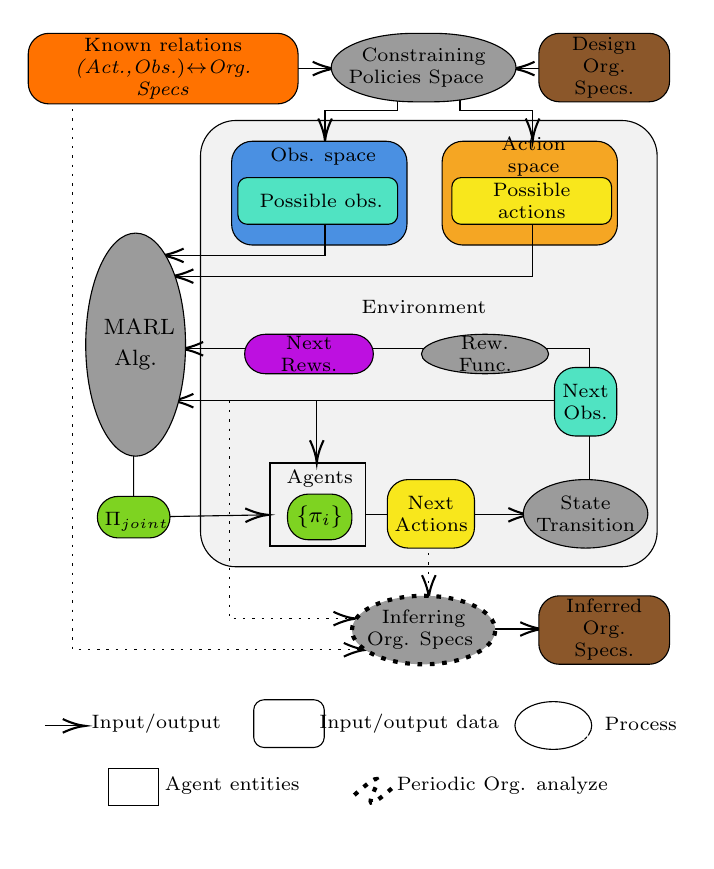
\begin{tikzpicture}[x=0.75pt,y=0.75pt,yscale=-1,xscale=1]
%uncomment if require: \path (0,1886); %set diagram left start at 0, and has height of 1886

%Shape: Rectangle [id:dp401980378305848] 
\draw  [fill={rgb, 255:red, 242; green, 242; blue, 242 }  ,fill opacity=1 ] (110,1267) .. controls (110,1257.61) and (117.61,1250) .. (127,1250) -- (313,1250) .. controls (322.39,1250) and (330,1257.61) .. (330,1267) -- (330,1448) .. controls (330,1457.39) and (322.39,1465) .. (313,1465) -- (127,1465) .. controls (117.61,1465) and (110,1457.39) .. (110,1448) -- cycle ;
%Straight Lines [id:da3175929748716908] 
\draw    (140.56,1440.03) -- (77.8,1441.11) -- (77.8,1396.11) ;
\draw [shift={(142.56,1440)}, rotate = 179.02] [color={rgb, 255:red, 0; green, 0; blue, 0 }  ][line width=0.75]    (10.93,-3.29) .. controls (6.95,-1.4) and (3.31,-0.3) .. (0,0) .. controls (3.31,0.3) and (6.95,1.4) .. (10.93,3.29)   ;
%Straight Lines [id:da6945547491407538] 
\draw    (297.41,1425) -- (297.41,1360) -- (102.33,1360) ;
\draw [shift={(100.33,1360)}, rotate = 360] [color={rgb, 255:red, 0; green, 0; blue, 0 }  ][line width=0.75]    (10.93,-3.29) .. controls (6.95,-1.4) and (3.31,-0.3) .. (0,0) .. controls (3.31,0.3) and (6.95,1.4) .. (10.93,3.29)   ;
%Straight Lines [id:da9008612661222812] 
\draw    (267.26,1440) -- (189.48,1440) ;
\draw [shift={(269.26,1440)}, rotate = 180] [color={rgb, 255:red, 0; green, 0; blue, 0 }  ][line width=0.75]    (10.93,-3.29) .. controls (6.95,-1.4) and (3.31,-0.3) .. (0,0) .. controls (3.31,0.3) and (6.95,1.4) .. (10.93,3.29)   ;
%Straight Lines [id:da7449421779677099] 
\draw    (166.02,1385) -- (166.02,1394.54) -- (166.02,1413) ;
\draw [shift={(166.02,1415)}, rotate = 270] [color={rgb, 255:red, 0; green, 0; blue, 0 }  ][line width=0.75]    (10.93,-3.29) .. controls (6.95,-1.4) and (3.31,-0.3) .. (0,0) .. controls (3.31,0.3) and (6.95,1.4) .. (10.93,3.29)   ;
%Rounded Rect [id:dp5816576242467624] 
\draw  [fill={rgb, 255:red, 245; green, 166; blue, 35 }  ,fill opacity=1 ] (226.41,1270) .. controls (226.41,1264.48) and (230.89,1260) .. (236.41,1260) -- (300.87,1260) .. controls (306.4,1260) and (310.87,1264.48) .. (310.87,1270) -- (310.87,1300) .. controls (310.87,1305.52) and (306.4,1310) .. (300.87,1310) -- (236.41,1310) .. controls (230.89,1310) and (226.41,1305.52) .. (226.41,1300) -- cycle ;
%Rounded Rect [id:dp9529058754609632] 
\draw  [fill={rgb, 255:red, 248; green, 231; blue, 28 }  ,fill opacity=1 ] (231.1,1282) .. controls (231.1,1279.51) and (233.12,1277.5) .. (235.6,1277.5) -- (303.56,1277.5) .. controls (306.04,1277.5) and (308.06,1279.51) .. (308.06,1282) -- (308.06,1295.5) .. controls (308.06,1297.99) and (306.04,1300) .. (303.56,1300) -- (235.6,1300) .. controls (233.12,1300) and (231.1,1297.99) .. (231.1,1295.5) -- cycle ;
%Straight Lines [id:da451152930226852] 
\draw    (283.33,1385) -- (97.63,1385) ;
\draw [shift={(95.63,1385)}, rotate = 360] [color={rgb, 255:red, 0; green, 0; blue, 0 }  ][line width=0.75]    (10.93,-3.29) .. controls (6.95,-1.4) and (3.31,-0.3) .. (0,0) .. controls (3.31,0.3) and (6.95,1.4) .. (10.93,3.29)   ;
%Straight Lines [id:da9734446377197741] 
\draw  [dash pattern={on 0.84pt off 2.51pt}]  (123.79,1385) -- (123.79,1490) -- (183,1490) ;
\draw [shift={(185,1490)}, rotate = 180] [color={rgb, 255:red, 0; green, 0; blue, 0 }  ][line width=0.75]    (10.93,-3.29) .. controls (6.95,-1.4) and (3.31,-0.3) .. (0,0) .. controls (3.31,0.3) and (6.95,1.4) .. (10.93,3.29)   ;
%Straight Lines [id:da9129668939660789] 
\draw    (164.39,1225) -- (125,1225) -- (173,1225) ;
\draw [shift={(175,1225)}, rotate = 180] [color={rgb, 255:red, 0; green, 0; blue, 0 }  ][line width=0.75]    (10.93,-3.29) .. controls (6.95,-1.4) and (3.31,-0.3) .. (0,0) .. controls (3.31,0.3) and (6.95,1.4) .. (10.93,3.29)   ;
%Straight Lines [id:da3918848581834071] 
\draw  [dash pattern={on 0.84pt off 2.51pt}]  (48.3,1240) -- (48.3,1505) -- (188,1505) ;
\draw [shift={(190,1505)}, rotate = 180] [color={rgb, 255:red, 0; green, 0; blue, 0 }  ][line width=0.75]    (10.93,-3.29) .. controls (6.95,-1.4) and (3.31,-0.3) .. (0,0) .. controls (3.31,0.3) and (6.95,1.4) .. (10.93,3.29)   ;
%Straight Lines [id:da46383821746892684] 
\draw    (285.34,1225) -- (262,1225) ;
\draw [shift={(260,1225)}, rotate = 360] [color={rgb, 255:red, 0; green, 0; blue, 0 }  ][line width=0.75]    (10.93,-3.29) .. controls (6.95,-1.4) and (3.31,-0.3) .. (0,0) .. controls (3.31,0.3) and (6.95,1.4) .. (10.93,3.29)   ;
%Straight Lines [id:da8847181725148201] 
\draw    (251.2,1495) -- (273,1495) ;
\draw [shift={(275,1495)}, rotate = 180] [color={rgb, 255:red, 0; green, 0; blue, 0 }  ][line width=0.75]    (10.93,-3.29) .. controls (6.95,-1.4) and (3.31,-0.3) .. (0,0) .. controls (3.31,0.3) and (6.95,1.4) .. (10.93,3.29)   ;
%Shape: Rectangle [id:dp08035475030295403] 
\draw   (143.5,1415) -- (189.48,1415) -- (189.48,1455) -- (143.5,1455) -- cycle ;
%Straight Lines [id:da24098465376222578] 
\draw    (205,1240) -- (205,1245) -- (170,1245) -- (170,1258) ;
\draw [shift={(170,1260)}, rotate = 270] [color={rgb, 255:red, 0; green, 0; blue, 0 }  ][line width=0.75]    (10.93,-3.29) .. controls (6.95,-1.4) and (3.31,-0.3) .. (0,0) .. controls (3.31,0.3) and (6.95,1.4) .. (10.93,3.29)   ;
%Shape: Boxed Line [id:dp8352454731616787] 
\draw    (35,1541.67) -- (52.58,1541.67) ;
\draw [shift={(54.58,1541.67)}, rotate = 180] [color={rgb, 255:red, 0; green, 0; blue, 0 }  ][line width=0.75]    (10.93,-3.29) .. controls (6.95,-1.4) and (3.31,-0.3) .. (0,0) .. controls (3.31,0.3) and (6.95,1.4) .. (10.93,3.29)   ;
%Shape: Rectangle [id:dp6328669951136969] 
\draw   (65.57,1562.23) -- (89.65,1562.23) -- (89.65,1580) -- (65.57,1580) -- cycle ;
%Curve Lines [id:da763384068727073] 
\draw [line width=1.5]  [dash pattern={on 1.69pt off 2.76pt}]  (184.12,1574.99) .. controls (212.34,1549.77) and (174.94,1596.12) .. (203.15,1570.9) ;

%Rounded Rect [id:dp3278199732714804] 
\draw  [fill={rgb, 255:red, 74; green, 144; blue, 226 }  ,fill opacity=1 ] (125,1270) .. controls (125,1264.48) and (129.48,1260) .. (135,1260) -- (199.47,1260) .. controls (204.99,1260) and (209.47,1264.48) .. (209.47,1270) -- (209.47,1300) .. controls (209.47,1305.52) and (204.99,1310) .. (199.47,1310) -- (135,1310) .. controls (129.48,1310) and (125,1305.52) .. (125,1300) -- cycle ;
%Rounded Rect [id:dp24054971346627085] 
\draw  [fill={rgb, 255:red, 80; green, 227; blue, 194 }  ,fill opacity=1 ] (128.04,1282) .. controls (128.04,1279.51) and (130.06,1277.5) .. (132.54,1277.5) -- (200.5,1277.5) .. controls (202.99,1277.5) and (205,1279.51) .. (205,1282) -- (205,1295.5) .. controls (205,1297.99) and (202.99,1300) .. (200.5,1300) -- (132.54,1300) .. controls (130.06,1300) and (128.04,1297.99) .. (128.04,1295.5) -- cycle ;
%Straight Lines [id:da12662032901914455] 
\draw    (92.94,1315) -- (170,1315) -- (170,1300) ;
\draw [shift={(90.94,1315)}, rotate = 0] [color={rgb, 255:red, 0; green, 0; blue, 0 }  ][line width=0.75]    (10.93,-3.29) .. controls (6.95,-1.4) and (3.31,-0.3) .. (0,0) .. controls (3.31,0.3) and (6.95,1.4) .. (10.93,3.29)   ;
%Straight Lines [id:da6903330894551778] 
\draw    (270,1300) -- (270,1325) -- (97.63,1325) ;
\draw [shift={(95.63,1325)}, rotate = 360] [color={rgb, 255:red, 0; green, 0; blue, 0 }  ][line width=0.75]    (10.93,-3.29) .. controls (6.95,-1.4) and (3.31,-0.3) .. (0,0) .. controls (3.31,0.3) and (6.95,1.4) .. (10.93,3.29)   ;
%Straight Lines [id:da5241788732296702] 
\draw  [dash pattern={on 0.84pt off 2.51pt}]  (220,1445) -- (220,1478) ;
\draw [shift={(220,1480)}, rotate = 270] [color={rgb, 255:red, 0; green, 0; blue, 0 }  ][line width=0.75]    (10.93,-3.29) .. controls (6.95,-1.4) and (3.31,-0.3) .. (0,0) .. controls (3.31,0.3) and (6.95,1.4) .. (10.93,3.29)   ;
%Shape: Boxed Line [id:dp4508196331907264] 
\draw    (235,1240) -- (235,1245) -- (270,1245) -- (270,1258) ;
\draw [shift={(270,1260)}, rotate = 270] [color={rgb, 255:red, 0; green, 0; blue, 0 }  ][line width=0.75]    (10.93,-3.29) .. controls (6.95,-1.4) and (3.31,-0.3) .. (0,0) .. controls (3.31,0.3) and (6.95,1.4) .. (10.93,3.29)   ;


% Text Node
\draw (168.17,1288.75) node  [font=\scriptsize] [align=left] {\begin{minipage}[lt]{45.19pt}\setlength\topsep{0pt}
\begin{center}
Possible obs.
\end{center}

\end{minipage}};
% Text Node
\draw (169.11,1267.5) node  [font=\scriptsize] [align=left] {\begin{minipage}[lt]{38.85pt}\setlength\topsep{0pt}
\begin{center}
Obs. space
\end{center}

\end{minipage}};
% Text Node
\draw  [fill={rgb, 255:red, 139; green, 87; blue, 42 }  ,fill opacity=1 ]  (273,1489) .. controls (273,1483.48) and (277.48,1479) .. (283,1479) -- (326,1479) .. controls (331.52,1479) and (336,1483.48) .. (336,1489) -- (336,1502) .. controls (336,1507.52) and (331.52,1512) .. (326,1512) -- (283,1512) .. controls (277.48,1512) and (273,1507.52) .. (273,1502) -- cycle  ;
\draw (304.5,1495.5) node  [font=\scriptsize] [align=left] {\begin{minipage}[lt]{40.43pt}\setlength\topsep{0pt}
\begin{center}
Inferred\\Org. Specs.
\end{center}

\end{minipage}};
% Text Node
\draw  [color={rgb, 255:red, 0; green, 0; blue, 0 }  ,draw opacity=1 ][fill={rgb, 255:red, 155; green, 155; blue, 155 }  ,fill opacity=1 ][dash pattern={on 1.69pt off 2.76pt}][line width=1.5]   (183,1495.5) .. controls (183,1486.39) and (198.45,1479) .. (217.5,1479) .. controls (236.55,1479) and (252,1486.39) .. (252,1495.5) .. controls (252,1504.61) and (236.55,1512) .. (217.5,1512) .. controls (198.45,1512) and (183,1504.61) .. (183,1495.5) -- cycle  ;
\draw (217.5,1495.5) node  [font=\scriptsize] [align=left] {\begin{minipage}[lt]{44.39pt}\setlength\topsep{0pt}
\begin{center}
Inferring\\Org. Specs \ \ 
\end{center}

\end{minipage}};
% Text Node
\draw  [fill={rgb, 255:red, 248; green, 231; blue, 28 }  ,fill opacity=1 ]  (200,1433) .. controls (200,1427.48) and (204.48,1423) .. (210,1423) -- (232,1423) .. controls (237.52,1423) and (242,1427.48) .. (242,1433) -- (242,1446) .. controls (242,1451.52) and (237.52,1456) .. (232,1456) -- (210,1456) .. controls (204.48,1456) and (200,1451.52) .. (200,1446) -- cycle  ;
\draw (221,1439.5) node  [font=\scriptsize] [align=left] {\begin{minipage}[lt]{26.14pt}\setlength\topsep{0pt}
\begin{center}
Next\\Actions
\end{center}

\end{minipage}};
% Text Node
\draw  [fill={rgb, 255:red, 126; green, 211; blue, 33 }  ,fill opacity=1 ]  (151.93,1440) .. controls (151.93,1434.48) and (156.41,1430) .. (161.93,1430) -- (172.93,1430) .. controls (178.45,1430) and (182.93,1434.48) .. (182.93,1440) -- (182.93,1442) .. controls (182.93,1447.52) and (178.45,1452) .. (172.93,1452) -- (161.93,1452) .. controls (156.41,1452) and (151.93,1447.52) .. (151.93,1442) -- cycle  ;
\draw (167.43,1441) node  [font=\footnotesize] [align=left] {\begin{minipage}[lt]{18.45pt}\setlength\topsep{0pt}
\begin{center}
$\displaystyle \{\pi _{i}\}$
\end{center}

\end{minipage}};
% Text Node
\draw (167.43,1422.5) node  [font=\scriptsize] [align=left] {\begin{minipage}[lt]{24.96pt}\setlength\topsep{0pt}
\begin{center}
Agents
\end{center}

\end{minipage}};
% Text Node
\draw  [fill={rgb, 255:red, 80; green, 227; blue, 194 }  ,fill opacity=1 ]  (280.53,1379) .. controls (280.53,1373.48) and (285.01,1369) .. (290.53,1369) -- (300.53,1369) .. controls (306.06,1369) and (310.53,1373.48) .. (310.53,1379) -- (310.53,1392) .. controls (310.53,1397.52) and (306.06,1402) .. (300.53,1402) -- (290.53,1402) .. controls (285.01,1402) and (280.53,1397.52) .. (280.53,1392) -- cycle  ;
\draw (295.53,1385.5) node  [font=\scriptsize] [align=left] {\begin{minipage}[lt]{17.81pt}\setlength\topsep{0pt}
\begin{center}
Next\\Obs.
\end{center}

\end{minipage}};
% Text Node
\draw  [fill={rgb, 255:red, 155; green, 155; blue, 155 }  ,fill opacity=1 ]  (173,1224.5) .. controls (173,1215.39) and (190.91,1208) .. (213,1208) -- (222,1208) .. controls (244.09,1208) and (262,1215.39) .. (262,1224.5) .. controls (262,1233.61) and (244.09,1241) .. (222,1241) -- (213,1241) .. controls (190.91,1241) and (173,1233.61) .. (173,1224.5) -- cycle  ;
\draw (217.5,1224.5) node  [font=\scriptsize] [align=left] {\begin{minipage}[lt]{57.49pt}\setlength\topsep{0pt}
\begin{center}
Constraining\\Policies Space \ \ \ 
\end{center}

\end{minipage}};
% Text Node
\draw  [fill={rgb, 255:red, 255; green, 114; blue, 0 }  ,fill opacity=1 ]  (27,1218) .. controls (27,1212.48) and (31.48,1208) .. (37,1208) -- (147,1208) .. controls (152.52,1208) and (157,1212.48) .. (157,1218) -- (157,1232) .. controls (157,1237.52) and (152.52,1242) .. (147,1242) -- (37,1242) .. controls (31.48,1242) and (27,1237.52) .. (27,1232) -- cycle  ;
\draw (92,1225) node  [font=\scriptsize] [align=left] {\begin{minipage}[lt]{85.61pt}\setlength\topsep{0pt}
\begin{center}
Known relations\\\textit{(Act.,Obs.})$\displaystyle \leftrightarrow $\textit{Org. Specs}
\end{center}

\end{minipage}};
% Text Node
\draw  [fill={rgb, 255:red, 189; green, 16; blue, 224 }  ,fill opacity=1 ]  (131.27,1362.5) .. controls (131.27,1357.25) and (135.74,1353) .. (141.27,1353) -- (183.27,1353) .. controls (188.79,1353) and (193.27,1357.25) .. (193.27,1362.5) .. controls (193.27,1367.75) and (188.79,1372) .. (183.27,1372) -- (141.27,1372) .. controls (135.74,1372) and (131.27,1367.75) .. (131.27,1362.5) -- cycle  ;
\draw (162.27,1362.5) node  [font=\scriptsize] [align=left] {\begin{minipage}[lt]{39.23pt}\setlength\topsep{0pt}
\begin{center}
Next Rews.
\end{center}

\end{minipage}};
% Text Node
\draw  [fill={rgb, 255:red, 155; green, 155; blue, 155 }  ,fill opacity=1 ]  (265.53,1439.5) .. controls (265.53,1430.39) and (278.97,1423) .. (295.53,1423) .. controls (312.1,1423) and (325.53,1430.39) .. (325.53,1439.5) .. controls (325.53,1448.61) and (312.1,1456) .. (295.53,1456) .. controls (278.97,1456) and (265.53,1448.61) .. (265.53,1439.5) -- cycle  ;
\draw (295.53,1439.5) node  [font=\scriptsize] [align=left] {\begin{minipage}[lt]{37.77pt}\setlength\topsep{0pt}
\begin{center}
State\\Transition \ 
\end{center}

\end{minipage}};
% Text Node
\draw  [fill={rgb, 255:red, 126; green, 211; blue, 33 }  ,fill opacity=1 ]  (60.3,1441.11) .. controls (60.3,1435.58) and (64.78,1431.11) .. (70.3,1431.11) -- (85.3,1431.11) .. controls (90.82,1431.11) and (95.3,1435.58) .. (95.3,1441.11) .. controls (95.3,1446.63) and (90.82,1451.11) .. (85.3,1451.11) -- (70.3,1451.11) .. controls (64.78,1451.11) and (60.3,1446.63) .. (60.3,1441.11) -- cycle  ;
\draw (77.8,1441.11) node  [font=\scriptsize] [align=left] {\begin{minipage}[lt]{20.95pt}\setlength\topsep{0pt}
\begin{center}
$\displaystyle \Pi _{joint}$
\end{center}

\end{minipage}};
% Text Node
\draw  [fill={rgb, 255:red, 155; green, 155; blue, 155 }  ,fill opacity=1 ]  (78.74, 1358) circle [x radius= 24.04, y radius= 53.74]   ;
\draw (78.74,1358) node  [font=\small] [align=left] {\begin{minipage}[lt]{23.12pt}\setlength\topsep{0pt}
\begin{center}
\phantom{x}\\{\footnotesize MARL}\\{\footnotesize Alg.}\\\phantom{x}
\end{center}

\end{minipage}};
% Text Node
\draw (269.58,1288.75) node  [font=\scriptsize] [align=left] {\begin{minipage}[lt]{54.32pt}\setlength\topsep{0pt}
\begin{center}
Possible actions
\end{center}

\end{minipage}};
% Text Node
\draw (270.52,1267.5) node  [font=\scriptsize] [align=left] {\begin{minipage}[lt]{43.61pt}\setlength\topsep{0pt}
\begin{center}
Action space
\end{center}

\end{minipage}};
% Text Node
\draw (216.23,1337.5) node  [font=\scriptsize] [align=left] {\begin{minipage}[lt]{42.81pt}\setlength\topsep{0pt}
\begin{center}
Environment
\end{center}

\end{minipage}};
% Text Node
\draw  [fill={rgb, 255:red, 155; green, 155; blue, 155 }  ,fill opacity=1 ]  (216.45,1362.5) .. controls (216.45,1357.25) and (230.16,1353) .. (247.08,1353) .. controls (264,1353) and (277.71,1357.25) .. (277.71,1362.5) .. controls (277.71,1367.75) and (264,1372) .. (247.08,1372) .. controls (230.16,1372) and (216.45,1367.75) .. (216.45,1362.5) -- cycle  ;
\draw (247.08,1362.5) node  [font=\scriptsize,xslant=-0.02] [align=left] {\begin{minipage}[lt]{38.44pt}\setlength\topsep{0pt}
\begin{center}
Rew. Func.
\end{center}

\end{minipage}};
% Text Node
\draw  [fill={rgb, 255:red, 139; green, 87; blue, 42 }  ,fill opacity=1 ]  (273,1218) .. controls (273,1212.48) and (277.48,1208) .. (283,1208) -- (326,1208) .. controls (331.52,1208) and (336,1212.48) .. (336,1218) -- (336,1231) .. controls (336,1236.52) and (331.52,1241) .. (326,1241) -- (283,1241) .. controls (277.48,1241) and (273,1236.52) .. (273,1231) -- cycle  ;
\draw (304.5,1224.5) node  [font=\scriptsize] [align=left] {\begin{minipage}[lt]{40.43pt}\setlength\topsep{0pt}
\begin{center}
Design\\Org. Specs.
\end{center}

\end{minipage}};
% Text Node
\draw (322.13,1540.49) node  [font=\small] [align=left] {{\scriptsize Process}};
% Text Node
\draw    (261.49,1541.49) .. controls (261.49,1535.13) and (269.77,1529.99) .. (279.99,1529.99) .. controls (290.21,1529.99) and (298.49,1535.13) .. (298.49,1541.49) .. controls (298.49,1547.84) and (290.21,1552.99) .. (279.99,1552.99) .. controls (269.77,1552.99) and (261.49,1547.84) .. (261.49,1541.49) -- cycle  ;
\draw (279.99,1541.49) node  [font=\small] [align=left] {\begin{minipage}[lt]{22.12pt}\setlength\topsep{0pt}
\begin{center}
\textcolor[rgb]{1,1,1}{{\tiny aassssaa}}
\end{center}

\end{minipage}};
% Text Node
\draw (88.72,1540.49) node  [font=\small] [align=left] {{\scriptsize Input/output}};
% Text Node
\draw (210.52,1540.49) node  [font=\small] [align=left] {{\scriptsize Input/output data}};
% Text Node
\draw    (135.63,1534.08) .. controls (135.63,1531.32) and (137.87,1529.08) .. (140.63,1529.08) -- (164.63,1529.08) .. controls (167.39,1529.08) and (169.63,1531.32) .. (169.63,1534.08) -- (169.63,1547.08) .. controls (169.63,1549.84) and (167.39,1552.08) .. (164.63,1552.08) -- (140.63,1552.08) .. controls (137.87,1552.08) and (135.63,1549.84) .. (135.63,1547.08) -- cycle  ;
\draw (152.63,1540.58) node  [font=\small] [align=left] {\begin{minipage}[lt]{20.08pt}\setlength\topsep{0pt}
\begin{center}
\textcolor[rgb]{1,1,1}{{\tiny assaaaa}}
\end{center}

\end{minipage}};
% Text Node
\draw (255.44,1570.49) node  [font=\small] [align=left] {{\scriptsize Periodic Org. analyze}};
% Text Node
\draw (125.31,1570.49) node  [font=\small] [align=left] {{\scriptsize Agent entities}};


\end{tikzpicture}
  \caption{Une vue récapitulative du processus PRAHOM}
  \label{fig:prahom_process}
\end{figure}

\subsubsection{Processus 1 : Déduire des spécifications organisationnelles}

Plutôt que d'utiliser directement les politiques conjointes, nous utilisons les historiques conjoints, car ils peuvent être construits avec les actions résultantes observées lorsque les observations sont reçues au cours d'une série d'épisodes de test. En effet, pour une politique donnée $\pi \in \Pi$, l'historique associé est par définition $h \in h_{joint} = \langle(\omega_k,a_k) | k \in \mathbb{N}\rangle$ et le $(\omega_k,a_k) \in \pi$.
Ensuite, en raison de la difficulté de déduire des informations liées aux spécifications organisationnelles, il est possible d'associer des séquences de couples observation-action aux spécifications de l'organisation sous la forme d'une relation \textquote{plusieurs à plusieurs}. Cela met en place un premier cadre d’identification des spécifications organisationnelles dans les historiques. Le reste de cette section aborde cette difficulté.

Le concepteur peut définir certaines relations entre les spécifications $\mathcal{M}OISE^+$ et les historiques conjoints. Leurs prémisses viennent du fait que certaines spécifications du modèle organisationnel $\mathcal{M}OISE^+$ peuvent être mappées à des sous-ensembles d'actions d'une seule politique commune sous-optimale.
À partir de ces relations, il est possible d’utiliser des approches empiriques ou statistiques pour déduire des spécifications organisationnelles à partir d’historiques communes.
%JS
%JPJ je te laisse reprendre au besoin. Penser a dire (si ce n'est pas fait) dans les perspective qu'il faudra lever cette hypothese -> Ça me va
Pour simplifier l'étude, nous ne considérons dans un premier temps qu'un seul groupe d'agents et nous ne prenons donc pas en compte les inter-liens et les inter-compatibilités. De même, nous ne considérons qu’un seul schéma social.
Premièrement, nous examinons le niveau individuel en essayant de comprendre les rôles, les liens, les sous-groupes, les objectifs individuels, les missions et les plans joués par les agents en échantillonnant les sous-séquences historiques $h \in H$ et en les comparant avec les sous-séquences historiques connues afin de déterminer des rôles.

Après avoir analysé plusieurs politiques conjointes, le processus tente de renforcer une vision globale des objectifs, des missions, des plans et de la connaissance de la mission par rapport à l'objectif ; avec les informations partiellement déduites au niveau individuel.
Au final, notre processus tente de synthétiser les connaissances inférées jusqu'à avoir une meilleure vision de la cardinalité des agents par sous-groupe, de la cardinalité des agents pour chaque mission, de la cardinalité des rôles, des compatibilités entre rôles, des autorisations et des obligations.

\subsubsection{Processus 2 : Contraindre l'espace des politiques}

Nous considérons un algorithme MARL donné qui converge itérativement vers une politique commune de sorte que la politique de chaque agent soit mise à jour à chaque étape jusqu'à un horizon fini.
Nous privilégions l'algorithme \emph{Proximal Policy Optimization} (PPO) pour son efficacité prouvée dans des environnements multi-agents coopératifs sans nécessiter de modifications algorithmiques ou d'architectures spécifiques au domaine~\cite{Yu2022}.
Pour contraindre les politiques conjointes possibles à celles satisfaisant les spécifications organisationnelles de conception $os_{init}$, nous proposons de contraindre les ensembles d'actions et d'observations pour chaque agent en fonction de $os_{init}$ à chaque étape. Par exemple, nous pouvons contraindre un agent à converger vers un rôle donné en interdisant les actions liées à d’autres rôles. Nous utilisons cette idée pour mettre en place notre processus visant à guider l'entrainement en fonction des contraintes organisationnelles de conception.

Dans un premier temps, nous utilisons les relations précédemment établies entre spécifications organisationnelles et couples action-observation, pour déterminer les actions autorisées ou interdites jouables par les agents à chaque étape.
Ensuite, il calcule d'abord l'ensemble d'actions autorisées $A_{step}$ en fonction de l'historique actuel $h_{joint,i}$. Ensuite, une action est choisie parmi les actions autorisées. Cette action $a_{step} \in A_{step}$ est ajoutée à l'historique pour être utilisée pour mettre à jour la politique de l'agent à l'étape suivante. Ensuite, l'algorithme MARL met à jour la politique commune, donc les politiques des agents, avec l'action et l'observation en cours.
Enfin, une analyse de la politique conjointe sous-optimale actuelle $\pi_{joint}$ satisfaisant $os_{init}$ est déclenchée périodiquement. Il permet d’améliorer de manière itérative l’efficacité des politiques conjointes et l’exactitude des spécifications organisationnelles qui en découlent.
Nous pouvons noter que la restriction impliquée par $os_{init}$ dans les éventuelles politiques conjointes pourrait empêcher l'algorithme MARL de trouver une politique commune qui satisfasse la récompense cumulative minimale attendue définie par le concepteur.

\subsection{Outil d'ingénierie}

%%%%%%%% DEBUT DES MODIFICATIONS %%%%%%%%%%%%%%
Dans le cadre de CybMASDE\footnotemark[1]
%
\footnotetext[1]{\emph{Cyberdefense Multi Agent System Developpment Environment} est un simulateur pour SMA de Cyberdéfense et disponible à \url{https://github.com/julien6/CybMASDE}}
%
, nous proposons \emph{PRAHOM Wrapper}\label{PettingZoo-wrapper} comme outil augmentant la bibliothèque \emph{PettingZoo} qui fournit une API standardisée pour le développement d'environnements et l'application d'algorithmes MARL.
%
\emph{PRAHOM Wrapper} fournit des moyens d'inférer des spécifications organisationnelles à partir d'agents entraînés ou contraindre leur entraînement.
% Lors de l'entraînement, des actions/observations sont masquées ou mis en avant pour contraindre l'apprentissage d'un agent selon les spécifications organisationnelles données.
%
\autoref{lst:wrapper_basic_use} présente une utilisation simple du wrapper pour augmenter un environnement \emph{PettingZoo} (ligne 5) avec des relations connues entre les spécifications organisationnelles et les historiques attendus (ligne 3) ainsi que les spécifications organisationnelles qui contraignent les politiques possibles des agents (ligne 4).

Ici, l'entrainement est effectué avec une fonctionnalité de \emph{PRAHOM Wrapper} qui utilise PPO et la configuration par défaut (ligne 6).
Pendant l'entrainement, \textquote{agent\_0} est contraint au rôle \textquote{follower}. Ainsi ses actions doivent être choisies d'après les historiques attendus (exprimables de diverses façons en plus de listes). Ces contraintes peuvent être satisfaites selon trois modes disponibles : i) masquer/corriger de façon externe aux politiques les observations reçues et actions choisies  ; ii) enseigner les contraintes aux politiques courantes ; iii) modifier en interne les politiques pour respecter les contraintes.

Après entrainement, \emph{PRAHOM Wrapper} infère les spécifications organisationnelles à partir de plusieurs historiques conjoints (lié chacun à un épisode) ; ainsi que l'instanciation de l'organisation généralisée pour chaque historique conjoint (ligne 7).
Ce processus d'inférence utilise d'abord les relations connues entre les historiques et les spécifications organisationnelles (ligne 3) : l'historique d'un agent qui contient l'observation $14$ (\textquote{commande reçue}) et l'action $74$ (\textquote{appliquer l’ordre}), est un \textquote{follower}. De même, pour les liens entre les rôles en utilisant des expressions régulières pour les historiques (ligne 3).
%
Ensuite, en s'appuyant sur la définition donnée de chaque spécification organisationnelle vis-à-vis des historiques, \emph{PRAHOM Wrapper} généralise plusieurs historiques conjoints.
% pour obtenir de nouvelles spécifications organisationnelles.
%
Par exemple, un rôle est obtenu en mesurant la similarité entre des historiques. Cela peut être fait de plusieurs manières : clustering de séquences (avec un dendrogramme) ; K-voisins les plus proches (avec ACP des historiques) ; analyse statistique (en particulier, fréquence d'action dans diverses visualisations) ; etc.

À partir des premières spécifications organisationnelles obtenues, un algorithme proposé déduit empiriquement d'autres spécifications organisationnelles telles que les compatibilités.
Ces résultats peuvent être incomplets ou bruités en raison des limites des techniques et de l'algorithme d'inférence des spécifications organisationnelles. Cependant, les résultats étant conformes à $\mathcal{M}OISE^+$, ils peuvent aider à la conception SMA à la lumière des spécifications organisationnelles proposées.
%%%%%%%% FIN DES MODIFICATIONS %%%%%%%%%%%%%%

\begin{lstlisting}[language=Python, caption={Utilisation basique de \emph{PRAHOM Wrapper}}, label={lst:wrapper_basic_use}]
from omarl_experiments import prahom_wrapper
env=PettingZoo_env.parallel_env(render_mode="human")
specs_to_hist={"structural_specifications":{"roles":{"follower":{"23":41,"14":[74,0]}}...},"functional_specifications":{"links":{"(leader,follower,aut)":".*14.*?89"}...}...}
policy_specs_constr={"agent_0":{"structural_specifications":"roles":["follower"]}}
env=prahom_wrapper(env,action_to_specs,training_specs)
env.train("default_PPO")
trained_specs,agent_to_specs=env.prahom_specs()
\end{lstlisting}

% =============

% \begin{itemize}
% \item Questions au niveau du système multi-agents (approche centrée sur le système)
% \begin{itemize}
% \item Nombre d'agents, quelle hétérogénéité ?
% \item Quel est le support commun (Environnement) partagé par les agents ?
% \item Quels mécanismes de communication sont disponibles pour les agents ?
% \item Quels sont les langages de communication, les ontologies, les protocoles d'interaction utilisés par les agents ?
% \item Quelle est l’organisation au sein de laquelle les agents opèrent ? Comment est-il établi ?
% \item Comment les agents coordonnent-ils leurs actions ? Comment assurer un fonctionnement cohérent ?
% \end{itemize}

% \item Questions au niveau de l'agent (approche centrée sur l'agent)
% \begin{itemize}
% \item Que représente un agent ? Quelles actions doivent être encapsulées dans un agent ?
% \item Comment les agents représentent-ils l'environnement et l'organisation dans lesquels ils opèrent ?
% \item Comment les agents gèrent-ils les interactions avec d'autres agents ?
% \item Quelle est la structure interne des agents ?
% \end{itemize}
% \end{itemize}

% ================================================== =================================================== =

\section{Évaluation dans des environnements de jeu coopératif}

% Évaluation
% Afin de vérifier et démontrer l'approche, est appliquée sur l'étude de cas suivante.
% 	Étude de cas

\subsection{Protocole expérimental}

Afin d'évaluer AOMEA, nous utilisons \emph{PRAHOM} dans des environnements simulés disponibles composés d'agents devant atteindre un objectif avec les meilleures performances à travers diverses stratégies collectives. Ces exemples présentent aussi l'avantage d'être facilement compréhensibles.
Nous avons sélectionné trois environnements de type Atari pour leur rendu visuel qui constitue un moyen pratique d'évaluer les résultats avec des observations manuelles\footnotemark[2].
Considérant la recherche sur les AICA, nous avons également considéré un environnement de Cyberdéfense comme une première tentative d'application de \emph{PRAHOM} dans un environnement de Cyberdéfense non "visuel" :

\footnotetext[2]{Des explications supplémentaires et les exemples discutés utilisant le \emph{PRAHOM Wrapper} sont disponibles sur \url{https://github.com/julien6/omarl_experiments?tab=readme-ov-file\#predator-prey-with-communication}}

\begin{itemize}
  \item \textquote{Drone swarm - 3rd CAGE Challenge}~\cite{cage_challenge_3_announcement} (CYB) se compose d'agents cyber-défenseurs déployés sur des drones en réseau essayant de lutter contre les programmes malware déployés de manière malveillante. Nous pouvons nous attendre à ce que les agents \allowbreak isolent collectivement les drones compromis ;
  \item \textquote{Pistonball} (PBL)~\cite{Terry2021} se compose d'une série de pistons pour amener une balle de droite à gauche, nécessitant ainsi la représentation des voisins ;
  \item \textquote{Predator-prey with communication}~\cite{Lowe2017} (PPY) se compose de prédateurs surveillés par un leader pour mieux attraper des proies plus rapides, nécessitant ainsi des stratégies de chasse collectives ;
  \item \textquote{Knights Archers Zombies}~\cite{Terry2021} (KAZ) consiste en trois chevaliers et deux archers apprenant à tuer le plus de zombies, ce qui nécessite ainsi un positionnement spatial efficace des agents.
\end{itemize}

Nous avons appliqué AOMEA dans trois cas :
\begin{itemize}
  \item Pas de spécifications organisationnelles (NTS) : les agents doivent apprendre les stratégies collectives les plus efficaces sans aucune contrainte ni indication.
  \item Spécifications organisationnelles partiellement contraignantes (PTS) : certaines contraintes ou indications sont données pour aider à converger plus rapidement ou à répondre à des exigences.
  \item Spécifications organisationnelles entièrement contraignantes (FTS) : des politiques conjointes élaborées manuellement sont données, car elles constituent une référence concernant les politiques conjointes apprises.
\end{itemize}

\

\noindent Ici, nous ne présentons pas le détail des contraintes données dans NTS et FTS (disponibles dans le référentiel Git\footnotemark[2]).
%
\begin{figure*}[h!]
  \centering
  \includegraphics[width=0.76\linewidth]{figures/prahom_learning_curve.png}
  \caption{Récompense moyenne pour chaque itération dans l'environnement PBL pour les cas NTS, PTS et FTS}
  \label{fig:prahom_learning_curve}
\end{figure*}
%
\begin{figure*}[h!]
  \centering
  \includegraphics[width=0.75\linewidth]{figures/prahom_pca_analysis.png}
  \caption{ACP des historiques des agents entrainés dans l'environnement PBL}
  \label{fig:prahom_pca_analysis}
\end{figure*}
%
Nous évaluons dans le tableau~\ref{tab:training_AOMEA_results}, l'impact de \emph{PRAHOM} sur les critères suivants : les ratios de temps de convergence entre PTS, NTS et FTS pour atteindre un seuil de récompense cumulée. La stabilité est le rapport entre la moyenne des récompenses cumulées sur la récompense maximale après plusieurs épisodes. La stabilité des performances montre si les agents atteignent l'objectif de façon générale en évaluant plusieurs environnements générés avec différents paramètres.

\begin{table}[t!]

    \centering

    \begin{tblr}{colspec={llll},rows={m},measure=vbox,stretch=-1}

        \textbf{Environment} & \textbf{Convergence time} & \textbf{} & \textbf{Stability} \\

        \hline

        { 1 }
        & {  }
        & {  } \\
        & {  } \\

        \hline[dashed]

        { 2 }
        & {  }
        & {  } \\
        & {  } \\

        \hline[dashed]

        { 3 }
        & {  }
        & {  } \\
        & {  } \\

        \hline[dashed]

        { 4 }
        & {  }
        & {  } \\
        & {  } \\

        \hline[dashed]

        { 5 }
        & {  }
        & {  } \\
        & {  } \\

    \end{tblr}

    \caption{View of the OOMARL approach impact during training}

    \label{tab:training_OOMARL_results}

\end{table}


\subsection{Analyse}

La \autoref{fig:prahom_learning_curve} montre l'évolution de la récompense dans les cas NTS, FTS et PTS pour l'environnement PBL. De manière générale, on peut remarquer que le temps de convergence est plus long pour NTS que pour PTS qui est également plus long que pour FTS. On constate, comme attendu, que l’espace de recherche diminuant, le temps de convergence est raccourci. Par exemple, nous remarquons une convergence plus rapide vers une solution sous-optimale dans l’environnement PBL en fournissant des spécifications organisationnelles. Bien que le PTS converge plus rapidement que le NTS vers une récompense cumulée comparable, le NTS peut surpasser le PTS parce que les politiques des agents entrainés sont conçues sur mesure pour résoudre le problème de manière beaucoup plus fine que ne peuvent les spécifications organisationnelles du concepteur. La faible stabilité des performances de l'environnement CYB indique que les agents ont des difficultés à trouver des stratégies générales à la différence des agents des autres environnements.

Nous prenons également en compte les critères suivants après l'entrainement : rôles, liens et performance globale. Une analyse qualitative est présentée dans le tableau~\ref{tab:trained_AOMEA_results}
%
\begin{table}[t!]

    \centering

    \begin{tblr}{colspec={llll},row{1}={rowsep=1mm,m},row{2-Z}={rowsep=0.5mm,m},measure=vbox,stretch=-10}

        \textbf{ \small Env.} & \textbf{ \small Rôles émerg.} & \textbf{ \small Links émerg.} & \textbf{\small Global \\ perf.} \\

        \hline

        { \small PBL }
        & { \small Claire émerg. \\ des rôles}
        & { \small Représentat° \\ locale }
        & { \small Proche de \\ optimal } \\

        \hline[dashed]

        { \small PPY }
        & { \small Différentat° \\ inhérente }
        & { \small Rares stratégies}
        & { \small Hautem\textsuperscript{t} \\ variable } \\

        \hline[dashed]

        { \small KAZ }
        & { \small Différentat° \\ inhérente }
        & { \small Représentat° \\ locale }
        & { \small Hautem\textsuperscript{t} \\ variable } \\

        \hline[dashed]

        { \small CYB }
        & { \small Emerg. roles \\ peu claire }
        & { \small Qques stratég-\\ies apparentes }
        & { \small Assez \\ bon } \\

    \end{tblr}

    \caption{Analyse qualitative des spécifications organisationnelles déduites après entrainement dans le cas NTS}

    \label{tab:trained_AOMEA_results}

\end{table}

%
% //TODO : schémas Moise+ et comparaison avec ceux attendus
%
Pour l'environnement PBL, les historiques des agents entrainés sont proches. Cela est visible dans l'ACP présentée à la \autoref{fig:prahom_pca_analysis} généré en exprimant les historiques des agents sous forme de vecteurs contenant les couples observation-action. Nous pouvons remarquer que l'historique de la plupart des agents se trouve dans la zone inférieure gauche (encerclée en rouge). Cela montre que la plupart des pistons semblent agir d'une façon similaire qu'on peut associer à un rôle. Nous ne pouvons déterminer aucune autre spécification organisationnelle en raison de l'absence de communication entre agents. Pour l'environnement KAZ, on peut remarquer deux rôles distincts : les archers ont tendance à s'éloigner des zombies, tandis que les chevaliers ont tendance à s'en approcher. Pour l'environnement PPY, nous pouvons observer que les spécifications de sortie indiquent des liens d'autorité entre le prédateur leader et les prédateurs simples pour permettre des stratégies collectives pour encercler les proies. Enfin, l’environnement CYB montre que les communications entre agents bleus permettent essentiellement d’isoler les drones suspectés ou de tenter de les réparer.

Pour l'environnement CYB, nous avons développé notre SMA raffiné via un simple arbre de décision élaboré à la main tel que préconisé dans AOMEA à la lumière des spécifications organisationnelles que nous obtenons en supprimant le bruit. Notre approche ne suggère pas de rôles généraux, mais des modèles stratégiques pertinents ont été identifiés. Par exemple, concernant les liens entre les rôles des agents, nous remarquons que les agents qui envoient des messages semblent fréquemment repérés comme suspects par leurs voisins. De plus, un agent cyber-défenseur se trouvant dans le rayon de communication d’un drone suspecté a tendance à couper sa communication et à la réactiver par la suite. Même si ces informations sont peu nombreuses, le score moyen que nous obtenons avec notre SMA affiné est d'environ -2000, ce qui est en effet proche des 5 meilleurs scores sur les 20 participants. Cela montre l'applicabilité d'AOMEA au contexte de la Cyberdéfense.

\section{Conclusion}

% Dans cet article, nous avons présenté AOMEA, une nouvelle approche générale de conception SMA qui vise à faciliter la conception SMA lorsqu'elle ne peut pas être facilement réalisée par les concepteurs dans des environnements de déploiement très complexes.
Les méthodes multi-agents s'appuient sur les connaissances du concepteur pour concevoir une organisation SMA adaptée, mais ne fournissent pas de moyens automatiques pour déterminer les mécanismes organisationnels pertinents.
% uniquement à partir des exigences de conception et de l'objectif global.
Les techniques MARL ont été appliquées avec succès pour entrainer automatiquement des agents à atteindre un objectif donné sans caractérisation explicite des stratégies collectives émergentes.
L'originalité d'AOMEA est d'enrichir un processus MARL d'un modèle organisationnel explicite vers un objectif méthodologique pour aborder ces problématiques. Nous avons d'abord exposé comment AOMEA est destiné à être utilisé dans l'ingénierie SMA en tant qu'outil supplémentaire pour aider au processus de conception.
Ensuite, nous avons proposé de lier les politiques des agents (modélisées dans un Dec-POMDP) avec $\mathcal{M}OISE^+$ à travers le processus \emph{PRAHOM} qui est au cœur d'AOMEA. Sous les conditions simplificatrices d'un groupe et d'un schéma social unique, \emph{PRAHOM} permet de déterminer partiellement les spécifications organisationnelles à partir des historiques conjoints et de contraindre l'entrainement des politiques par rapport à des spécifications organisationnelles.
De plus, nous avons implémenté le wrapper \emph{PRAHOM PettingZoo} comme preuve de concept pour appliquer AOMEA.
Enfin, nous avons appliqué notre approche dans quatre environnements \emph{PettingZoo} pour évaluer l'impact pendant et après l'entrainement. Les performances obtenues se révèlent comparables à ceux connus.

Même si \emph{PRAHOM} est agnostique à l'égard de l'algorithme MARL, car il utilise l'historique des agents pour déduire des spécifications organisationnelles, reconstruire a posteriori les comportements collectifs des agents peut s'avérer difficile. En effet, une perspective majeure pour améliorer \emph{PRAHOM} est d'aller plus loin avec les techniques d'apprentissage non supervisé en plus des approches statistiques empiriques pour identifier des spécifications organisationnelles pertinentes à partir d'historiques conjoints. De plus, les travaux issus de l’apprentissage hiérarchique peuvent contribuer à mieux caractériser les stratégies émergentes durant l’apprentissage.
%À terme, nous visons également à améliorer l'applicabilité d'AOMEA en développant des interfaces dédiées construites autour de \emph{PRAHOM} le rendant plus accessible aux contextes industriels et de recherche.


% \begin{thebibliography}{9}
% {\small
% \bibitem{bar} U. Nexpert, \emph{Le livre,} Son Editeur, 1929.

% \bibitem{foo} I. Troiseu-Pami, Un article intéressant, \emph{Journal de
%     Spirou}, Vol. 17, pp. 1-100, 1987
% }
% \end{thebibliography}
\section*{Remerciements}

Ce travail est financé par \emph{Thales Land Air Systems} dans le cadre des travaux conjoints de la chaire \emph{Cyb'Air} et de l'\emph{AICA IWG}.

\section*{References}
\small
\bibliographystyle{plain}
\bibliography{references}


\end{document}

%%% Local Variables: 
%%% mode: latex
%%% TeX-SMAter: "jfsmaLatex"
%%% ispell-local-dictionary: "francais"
%%% TeX-command-extra-options: "-shell-escape"
%%% End: 